\newpage
%\vspace{2em}
\section{Omówienie celu naukowego wyżej wymienionych prac, osiągniętych wyników oraz ich ewentualnego wykorzystania}\vspace{-1em}
Duży odsetek publikacji w tematyce systemów nadzorowanego uczenia się maszyn rozpoczynany jest parafrazą zdania \emph{"współczesny świat wypełniony jest danymi"}. Przyczynia się do tego wiele postępujących czynników, rozpoczynając od tak pozytywnych zjawisk jak masowa digitalizacja treści\citeZ[-5.5em]{Z1}, automatyzacja procesów produkcyjnych\citeZ[-1em]{Z2} czy rosnąca rola  systemów rekomendacyjnych~\citeZ[.5em]{Z3}. 

Należy jednak zwrócić również uwagę na bardziej złożone społecznie zjawiska takie jak popularyzacja wykorzystania pojazdów autonomicznych, w tym w usługach kurierskich i transportowych redukujących czynnik ludzki\citeZ[.5em]{Z4}, spadająca jakość produktów elektronicznych powodująca zwiększoną potrzebę automatycznych systemów diagnostyki sprzętu\citeZ[.5em]{Z5}, modelowanie zachowań ludzkich i -- szczególnie niepokojące -- profilowanie konsumentów w świecie, w którym dominująca większość naszych zachowań pozostawia swój ślad cyfrowy\citeZ[.5em]{Z6}. Proces ten wzmacniany jest także przez trwającą nieprzerwanie od końca \oldstylenums{2019} roku pandemię wirusa \emph{SARS-CoV-2}, który w dniu finalnej redakcji tego dokumentu dotknął bezpośrednio już ponad pół miliarda mieszkańców Ziemi, stanowiąc dodatkowy, niezaprzeczalny argument za automatyzacją czynności i procedur, które dotychczas wykonywane były przez odpowiednio wyszkolonych do tego celu ludzi.

Już w latach siedemdziesiątych zauważone zostało, zarówno w krytycznym dla całego środowiska maszyn uczących się raporcie Lighthilla\citeZ{Z7}, jak i w merytorycznych ocenach ówczesnego stanu badań nad systemami sztucznej inteligencji\citeZ[.5em]{Z8}, że indukcyjne modele predykcyjne najlepiej radzą sobie z problemami opisywanymi przez stosunkowo niewielką liczbę atrybutów. Przy silnie ograniczonej mocy obliczeniowej komputerów tamtej epoki\citeZ[.5em]{Z9}, większość publikacji opierała zawarte w nich obserwacje na temat efektywności poszczególnych metod rozpoznawania na tzw. \emph{toysetach} (zbiorach ilustracyjnych), ograniczonych do zaledwie kilku wymiarów i opisanych przez nie więcej niż kilkaset instancji. Ograniczenia te istotnie utrudniały generalizację wniosków na problemy rzeczywiste, opisywane przez potencjalnie nieskończone zbiory danych o wysokiej liczbie atrybutów.

Metody uczenia nadzorowanego, zgodnie z powszechnie przyjętą taksonomią, skupiają się na zadaniach regresji i klasyfikacji\citeZ{Z10}. W~pierwszym z tych przypadków rolą systemu rozpoznawania jest zyskanie zdolności do wyznaczania, najczęściej ciągłej, wartości zmiennej objaśnianej na podstawie zbioru odpowiednio anotowanych obserwacji. W~zadaniu klasyfikacji -- na którym skupia się większość prowadzonych przeze mnie badań -- obiekty przypisywane są do jednej z predefiniowanych kategorii nazywanych klasami problemu. W wypadku rzeczywistych zbiorów danych dla zadania klasyfikacji stosunkowo rzadka jest sytuacja, w której dysponujemy równomierną reprezentacją każdej z tych kategorii, co przynosi dodatkową trudność w ich analizie\citeZ[-7em]{Z11}. Trudność ta jest na tyle silna, że pozwoliła na wyodrębnienie się istotnego nurtu badań nad klasyfikacją danych niezbalansowanych\citeZ[-4.5em]{Z12}.

Modele klasyfikacji, często niezależnie od rodziny z której pochodzą, wykazują silną tendencję do faworyzowania decyzji w kierunku klasy dominującej zbiór danych\citeZ[-1.5em]{Z13}. Przykładowo, reguły splitu drzew decyzyjnych, przypisując etykietę do wierzchołka budowanego grafu uwzględniają przede wszystkim proporcję pomiędzy etykietami zakreślonych jego parametrami obiektów\citeZ[-.5em]{Z14}. Funkcje straty wykorzystywane w trenowaniu sieci neuronowych najczęściej tym samym kosztem obciążają błędne decyzje względem każdej z klas problemu\citeZ[.5em]{Z15}. Wreszcie, proste podejścia do rozpoznawania takie jak klasyfikatory minimalnoodległościowe, również wykazują tendencję do premiowania obiektów klas o większym prawdopodobieństwie \emph{a priori}, co w każdym z wymienionych przypadków prowadzi do budowy modeli nadmiernie ograniczających obszar decyzyjny klasy mniejszościowej~\citeZ[-1em]{Zyb19}.

Najpowszechniej występujące współcześnie trudności przetwarzania danych powiązane są z czynnikiem ich masowości, dokładniej opisywanym przez model 4V Big Data\citeZ[.5em]{Z16}. Masowość danych wyrażać może się zarówno we wspomnianym już kontekście wielowymiarowości, jak też w niezwykle dużej liczności zbiorów. Pierwotną motywacją badań w tym zakresie były ograniczenia obliczeniowe i pamięciowe maszyn z drugiej połowy \textsc{xx} wieku, które nie pozwalały ani na jednoczesne składowanie pełnego zbioru danych, ani na przetworzenie wszystkich dostępnych wzorców w akceptowalnym czasie obliczeniowym\citeZ[-1em]{Z17}. Podstawowe rozwiązania w tym zakresie wprowadzają paradygmat tzw.~uczenia inkrementalnego, dostępny zarówno dla prostych modeli takich jak \emph{Naive Bayes} czy niektóre drzewa decyzyjne\citeZ[.5em]{Z18}, jak i dla złożonych procedur optymalizacyjnych, wśród których największy nacisk należałoby położyć na sieci neuronowe~\citeZ{Z19}.

Typowy przypadek uczenia inkrementalnego, podobnie jak bardziej ogólna koncepcja \emph{i. i. d.} (ang. \emph{independent and identically distributed}) stanowiąca kluczowe zagadnienie walidacji modeli rozpoznawania, opiera się na założeniu o stacjonarności koncepcji, tj. na niezmienności prawdopodobieństwa \emph{a~posteriori} problemu. Dzięki takiemu założeniu, algorytm uczenia pozwalający na aktualizację wiedzy otrzymuje w każdym kroku wsad z dostępnych danych uczących -- w zależności od zastosowanego podejścia rozłączny lub losowy -- i dokonuje korekty modelu na ich podstawie. Korekta ta uwzględnia fakt, że systemowi rozpoznawania dostarczone zostały już wcześniej pewne przykłady opisujące problem i z czasem rola nowych obiektów jest coraz mniejsza, pozwalając na konwergencję modelu~\citeZ{Z20}.

Dziedzina przetwarzania strumieni danych rozwija paradygmat uczenia inkrementalnego o uwzględnienie czynnika czasu przez uznanie zbioru obiektów za uporządkowaną sekwencję. Daje to zarówno podstawę do właściwego spojrzenia na prędkość przetwarzania danych -- ponieważ obserwacje opisywane są i w czasie i przestrzeni -- jak i rozszerzenie pojęcia różnorodności poza heterogeniczność źródeł, przez zniesienie założenia o stacjonarności koncepcji. Procedury uczenia w~takim środowisku muszą ulegać zmianie i nie dążyć już do analizy stabilnego zjawiska, ale do konsekwentnej modyfikacji założeń na jego temat, znajdujących odzwierciedlenie w modelu zdolnym do śledzenia dynamiki jego zmian~\citeZ[-3em]{Z21}. 

Zmiany tego rodzaju zwykło się w literaturze nazywać dryfami lub dryftami koncepcji (ang. \emph{concept drift})~\citeZ[-2em]{Z22}. W uproszczonej taksonomii możemy wyróżnić dryfy wirtualne -- zmieniające co prawda rozkład klas w przestrzeni, ale nie mające istotnego wpływu na zmiany we właściwej granicy decyzyjnej oraz dryfy rzeczywiste -- stanowiące podstawowe źródło czasowej degeneracji modeli i najczęściej spotykane w strumieniach rzeczywistych. Degeneracja modelu może być również tymczasowym spadkiem jego zdolności generalizacyjnej, w wypadku strumieni o koncepcjach nawracających (ang. \emph{recurrent drift}), typowych dla danych opisujących zjawiska okresowe o uporządkowanej (cykl dobowy, cykl roczny) lub nieuporządkowanej (pogoda, rynek giełdowy) naturze.

\vspace{-.5em}\noindent \newthought{Podział cyklu publikacji na obszary tematyczne}~\\
\noindent Od roku złożenia rozprawy doktorskiej, która podejmowała tematykę metod reprezentacji i klasyfikacji danych wielowymiarowych, w~swoich pracach badawczych stale rozwijam metody pozwalające na efektywne przetwarzanie danych obciążonych wymienionymi wyżej trudnościami. Biorąc je pod uwagę, do typowego dla wstępów do prac z dziedziny stwierdzenia o tym, że \emph{świat wypełniony jest danymi}, warto byłoby dodać informację, iż dane te -- tak samo jak świat, który opisują -- ulegają ciągłym zmianom, a efektywne systemy rozpoznawania powinny być zdolne do ich rejestrowania i nadążania za nimi.

W kolejnych sekcjach opiszę zaproponowane przeze mnie metody oraz towarzyszące im publikacje, wpisujące się w opisaną tematykę i~będące podstawą osiągnięcia naukowego. Listę jedenastu artykułów naukowych stanowiących opisywany cykl wpisałem w trzy przenikające się kategorie:

\begin{enumerate}
	\item[\emph{I}] Algorytmy przetwarzania danych wielowymiarowych.
	\item[\emph{II}] Algorytmy przetwarzania danych niezbalansowanych.
	\item[\emph{III}] Algorytmy przetwarzania strumieni danych.
\end{enumerate}

\begin{figure}[h]
	\centering
	\scalebox{.6}{\large
	\def\imbcircle{(-210:2) circle (2.725cm)}
	\def\dscircle{(-330:2) circle (2.725cm)}
	\def\mdcircle{(-90:2) circle (2.725cm)}

	\begin{tikzpicture}
		%\draw[step=1.0,black,thin,dotted] (-5,-5) grid (5,5);
      	\begin{scope} % W miarę
    		%\clip \firstcircle;
    		%\fill[green!25] \mdcircle;
      	\end{scope}
      	\begin{scope} % W miarę
    		%\clip \firstcircle;
    		%\fill[yellow!25] \imbcircle;
      	\end{scope}
      	\begin{scope} % Git
    		%\clip \firstcircle;
    		%\fill[green!25] \dscircle;
      	\end{scope}
      	\begin{scope} % Problematyczny
    		%\clip \dscircle;
    		%\fill[red!25] \mdcircle;
      	\end{scope}
      	
      	\node[fill=black,rotate=-210-90, text width=5.25cm, text height=2.9cm] at (-210:3.625) {};
      	\node[fill=black,rotate=-330-90, text width=5.25cm, text height=2.9cm] at (-330:3.625) {};
      	\node[fill=black,rotate=0, text width=5.25cm, text height=2.9cm] at (-90:3.625) {};
      	
      	\node[color=white,fill=black,rotate=-210-90,rounded corners=.25cm, text width=5.25cm, align=center] at (-210:5.25) {\bfseries \textsc{dane niezbalansowane}};
      	\node[color=white,fill=black,rotate=-330-90,rounded corners=.25cm, text width=5.25cm, align=center] at (-330:5.25) {\bfseries \textsc{strumienie danych}};
		\node[color=white,fill=black,rotate=0,rounded corners=.25cm, text width=5.25cm, align=center] at (-90:5.25) {\bfseries \textsc{dane wielowymiarowe}};


    	\draw[fill=white] \imbcircle;
      	\draw[fill=white] \dscircle;
      	\draw[fill=white] \mdcircle;

      	
    	\draw[ultra thick] \imbcircle;
      	\draw[ultra thick] \dscircle;
      	\draw[ultra thick] \mdcircle;
      	

      	%\node[fill=white,rotate=-210-90,rounded corners=.25cm, text width=3cm, align=center] at (-210:4.5) {\bfseries Dane\\Niezbalansowane};
      	%\node[fill=white,rotate=-330-90,rounded corners=.25cm] at (-330:4.5) {\bfseries DS};
      	%\node[fill=white,rotate=-90+90,rounded corners=.25cm] at (-90:4.5) {\bfseries MD};
      	
      	% IMB
      	\node at (-210:3) {[C6]}; %7
      	
      	% IMB + DS
      	\node at (90:1.75) {[C3]};
      	\node at (90:1.25) {[C4]}; % 6
      	
      	% DS
      	\node at (-330:2.5) {[C7]};
      	\node at (-330:3.5) {[C1]};
      	
      	% MD
      	\node at (-90:2.5) {[C11]}; % 11
      	\node at (-90:3.5) {[C10]}; % 15
    
    	% IMB + MD
      	\node at (-330-180:1.25) {[C9]}; % 14
      	\node at (-330-180:2) {[C8]}; % 19
      	%\node at (-330-180:2.25) {[C10]}; % 19  	
      	
      	% DS + MD
      	\node at (-210-180:1.25) {[C5]};
      	
      	% ALL
      	\node at (0:0) {[C2]};
	\end{tikzpicture}}
	\caption{Przypisanie prac z cyklu publikacji do zakresu tematycznego klasyfikacji danych trudnych. Podane w nawiastach kwadratowych indentyfikatory odwołują się do spisu zawartego w P4.}\label{fig:philips}
\end{figure}

Przypisanie poszczególnych prac do kategorii zostało zilustrowane w~Rysunku~\ref{fig:philips} zawierającym nachodzące na siebie obszary badawcze wraz ze stosownymi odniesieniami literaturowymi.

\subsection*{I -- Algorytmy przetwarzania danych wielowymiarowych}

\marginnote{\scalebox{.6}{\large
	\def\imbcircle{(-210:2) circle (2.725cm)}
	\def\dscircle{(-330:2) circle (2.725cm)}
	\def\mdcircle{(-90:2) circle (2.725cm)}

	\begin{tikzpicture}
      	
      	\node[fill=black,rotate=0, text width=5.25cm, text height=2.9cm] at (90:-.5) {};
		\node[color=white,fill=black,rotate=0,rounded corners=.25cm, text width=5.25cm, align=center] at (90:1.25) {\bfseries \textsc{dane wielowymiarowe}};
      	
      	\draw[fill=white] \mdcircle;
      	\draw[ultra thick] \mdcircle;
      	
      	% 10 9 11 
      	% MD
      	\node at (-90:.5) {[C11]};
      	\node at (-90:1.25) {[C10]};    
      	\node at (-90:2.0) {[C9]};
      	%\node at (-330-180:1.75) {[4]};
      	      	   
      	\node at (-90:2.75) {\color{black!50}\emph{[C8]}};   
      	\node at (-90:3.5) {\color{black!50}\emph{[C2]}};
      	% DS + MD
      	%\node at (-210-180:1.25) {[5]};
      	%\node at (-210-180:1.75) {[6]};
      	
      	% ALL
      	%\node at (0:0) {[7]};
	\end{tikzpicture}}}

Po prawej stronie diagram zaznaczający opisywane w ramach wątku przetwarzania danych wielowymiarowych, wliczający prace opisane w~innych wątkach dominujących.

Najsilniej rozwijającą się w ostatnim dziesięcioleciu odpowiedzią środowiska naukowego na stale rosnącą wymiarowość danych jest bez wątpienia nurt uczenia reprezentacji (ang. \emph{representation learning}). Dedykowany jest on głównie wielowymiarowym danym sygnałowym, w których najczęściej spotykamy bardzo silne, ale jednocześnie zmienne, relacje pomiędzy atrybutami, stanowiącymi najczęściej wartości poszczególnych elementów obrazu.

Niemniej jednak, nadal interesującą alternatywą są tutaj metody klasyczne, uwzględniające element manualnej inżynierii cech. Pozwalają one na wstępną redukcję atrybutów, które łatwiej jest opisać przez podprzestrzenną dywersyfikację nowej przestrzeni, konstruując tak już dwupoziomowy system rozpoznawania zdolny do budowy złożonych granic decyzyjnych nawet przy użyciu prostych klasyfikatorów bazowych.

Szczególnym przypadkiem obrazów cyfrowych są \emph{obrazy nadwidmowe}\footnote{W j. polskim brak jest powszechnie uznanej taksonomii dla danych o~ciągłym wymiarze spektralnym, w~związku z~czym posługuję się tutaj tłumaczeniem wykorzystywanym w~raportach sprawozdawczych, zaproponowanym w 2014 roku.} (ang. \emph{hyperspectral images}). Stanowią one efekt próbkowania promieniowania elektromagnetycznego zarówno w dwóch wymiarach przestrzennych -- jak standardowe obrazy -- jak i w wymiarze spektralnym, dzięki zastosowaniu pryzmatu rozszczepiającego promieniowanie elektromagnetyczne na wąskie, rozłączne pasma opisujące zakres częstotliwości przekraczający zdolność widzenia ludzkiego\footnote{Na przykładzie sensora \textsc{aviris}.}. W sytuacji, w której liczba takich pasm przekracza setkę, zbiór atrybutów dla każdego piksela przestaje być pulą luźno powiązanych ze sobą czynników (jak w reprezentacji \textsc{rgb} czy obrazach wielowidmowych) i staje się już typową dla obrazu nadwidmowego sygnaturą spektralną.

Stanowi to niezwykle interesujący przypadek danych rzeczywistych, w~których możemy mówić o ciągłości informacji w~każdym z~wymiarów obrazu. Sygnatura spektralna, którą najczęściej wykorzystujemy~w badaniach jako bazową reprezentację wzorca, jest jednowymiarowym sygnałem cyfrowym zbliżonym w~swoim przebiegu do wyraźnie zaszumionego wykresu funkcji wielomianowej. Szum ten najczęściej ma charakter globalny w~skali obrazu i typowy dla wykorzystanego sensora.

Dane nadwidmowe reprezentowane są przez tzw. \emph{kostki hiperspektralne} (ang. \emph{hyperspectral cubes}) będące trójwymiarowymi tensorami, które dla zadania klasyfikacji uzupełnione są o dwuwymiarową, dyskretną mapę \emph{ground truth}, tj. etykiet każdego piksela. Prezentują one najczęściej zdjęcia lotnicze pól uprawnych i~miast, budując wieloklasowe problemy niezbalansowane, choć zakres ich zastosowań wykracza też poza tę specyfikę i~odnajduje się -- przykładowo -- w obrazowaniu palimpsestów i~kontroli jakości produkcji.\vspace{1em}

{
\color{red}
\noindent\begin{tabular}{p{\textwidth}}
	\toprule &
\end{tabular}\vspace{-1em}
}
\noindent W \citeC[-2.25em]{C10} zaproponowałem autorską metodę budowy systemu rozpoznawania dla obrazów nadwidmowych, opartą o ręczną inżynierię atrybutów i zespołową integrację szybkich sieci neuronowych \emph{Extreme Learning Machines} (\textsc{elm}).

Silna zależność pomiędzy cechami zawartymi w~sygnaturze spektralnej powiązana jest z~równie silną nadmiarowością zapisanej w~niej informacji. Strategią przeciwdziałającą redundancji jest zerwanie ciągłości widmowej danych, którą możemy uzyskać przez selekcję atrybutów lub ich ekstrakcję. W selekcji jest to często operacja silnie stratna i~wzmacniająca rolę szumu w~pojedynczej próbce, a~w~ekstrakcji i~uczeniu reprezentacji -- gubiąca interpretowalność atrybutów. Alternatywą jest tutaj, wzorowana na właściwościach fotoreceptorów, ręczna inżynieria atrybutów, gdzie każda nowa cecha stanowi liniową kombinację elementów sygnatury bazowej, posiada swoją semantyczną interpretację i~wykazuje obniżoną zależność od pozostałych.

Zaproponowałem tu czternaście metryk statystycznych rozpinających się od prostych miar, takich jak minimum, średnia czy mediana sygnatury, przez metryki zróżnicowania sygnału reflektancji, interpretowanego jako zmienna losowa po pseudo kanały barwne uzyskane z projekcji całego obrazu do modelu \textsc{hsv}.

Należy mieć tu na uwadze, że inżynieria atrybutów oparta na miarach statystycznych jest nadal silnie czuła na błędy pomiarów, które są szczególnie widoczne w rzeczywistych obrazach nadwidmowych. Do~przeciwdziałania ich negatywnym skutkom wykorzystałem, zaproponowany przeze mnie w jednej z wcześniejszych prac, \emph{Entropodynamiczny Filtr Percentylowy}~\citeM{Ksi18e}, który pozwala na detekcję impulsywnych zmian sygnału i tym samym oznaczenie pasm sygnatury obciążonych wysokim błędem -- zakłócającym wartości metryk statystycznych.

Kluczowym zagadnieniem pracy było odpowiednie wykorzystanie potencjału algorytmu \textsc{elm}. Jego model neuronowy jest silnie oparty na losowości, pozwalając na~znacznie krótszy proces uczenia niż \textsc{mlp}, jednak kosztem znacznie wyższej wariancji modelu. Stabilizacja takiego rozwiązania często realizowana jest przez wykorzystanie uczenia zespołowego (ang. \emph{ensemble learning}), czego skuteczność została już potwierdzona w~wielu publikacjach~\citeZ[-3em]{Z23}. Krytyczny dla zespołu aspekt dywersyfikacji jego puli najczęściej opiera się na~losowości wag wejściowych, co~przy szerokim i silnie zależnym wewnętrznie wektorze atrybutów zdecydowanie nie jest rozwiązaniem optymalnym. Literatura pokazuje, że~dla danych tego typu znacznie lepszą strategią jest dywersyfikacja projekcyjna~\citeZ[-4.5em]{Z24} lub podprzestrzenna~\citeM[.5em]{Sul21}, która możliwa jest~do efektywnego zastosowania -- przykładowo -- po zaproponowanej ręcznej inżynierii cech. 

W wypadku dywersyfikacji podprzestrzennej (ang. \emph{random subspace}) musimy pamiętać o~zapewnieniu pełnego pokrycia oryginalnej przestrzeni atrybutów. Prawdopodobieństwo pokrycia możemy wyliczyć przez wzór:

\begin{equation}
	P(coverage) = 1 - (1-\frac{r}{d})^L,
\end{equation}

\noindent gdzie $r$ to wielkość podprzestrzeni, $d$ -- liczba atrybutów, a $L$ to wielkość puli. Naturalnie, przy zachowaniu stałej wielkości podprzestrzeni $r$, wraz ze wzrostem liczby wymiarów problemu powinniśmy też proporcjonalnie zwiększać pulę modeli, pamiętając jednak o tym, że po przekroczeniu pewnego limitu będzie ona wpływać negatywnie na różnorodność.

Przy wykorzystaniu 14. atrybutów statystycznych zamiast ponad 200. spektralnych\sidenote[]{Najczęściej wykorzystywany w danych benchmarkowych sensor \textsc{aviris} opisuje 224 pasma w widmie od 400 do 2 500 nanometrów.} możliwe jest więc zbudowanie mniejszego zespołu klasyfikatorów dywersyfikowanego przez \textsc{rsm} pozwalającego na pełne pokrycie przestrzeni atrybutów.

Zespoły \textsc{elm} domyślnie integruje się przez reguły głosowania większościowego, co daje duży potencjał do modyfikacji mających istotny wpływ na jakość docelowego modelu. W pracy proponuję więc komplementarnie ważoną integrację zespołu, gdzie za wyliczenie optymalnych wag -- dla każdej klasy indywidualnie -- odpowiada pojedynczy perceptron.

Uzyskane rezultaty badań pozwoliły na uprawdopodobnienie hipotezy stanowiącej o tym, że zespołowy model \textsc{elm} dywersyfikowany przez \textsc{rsm} z wykorzystaniem atrybutów statystycznych, integrowany z~wykorzystaniem wyuczalnej reguły decyzyjnej okazuje się statystycznie istotnie lepszy od podejść standardowych dla większości analizowanych zbiorów danych. Możemy dzięki nim zaobserwować też, że odpowiednia selekcja atrybutów, bez wykorzystywania metod wbudowanych czy resamplingu, może prowadzić do istotnego statystycznie ulepszenia modelu klasyfikacji nawet w wieloklasowych danych niezbalansowanych.\vspace{1em}

{
\color{red}
\noindent\begin{tabular}{p{\textwidth}}
	\toprule &
\end{tabular}\vspace{-1em}
}
\noindent Obserwacja ta stała się podstawą do badań przedstawionych w \citeC[-2.25em]{C9}. Stanowią one analizę odchodzącą już od specyfiki obrazów nadwidmowych, gdzie ewaluacja przeprowadzona została na kolekcji 35 tabelaryczych zbiorów o skali niezbalansowania sięgającej 1:41. 

Należy zaznaczyć, że punktem wyjściowym badań było wykorzystanie problemów o wstępnie zredukowanej wymiarowości -- przyjmując przestrzenie od 8 do 19 atrybutów -- i analiza potencjału metod optymalizacyjnych w selekcji podprzestrzeni do ulepszenia efektywności w~klasyfikacji niezbalansowanej.

W artykule zaproponowałem autorską metodę hybrydową wykorzystującą techniki selekcji atrybutów do budowy puli klasyfikatorów na potrzeby zespołu. Celem uniknięcia przeuczenia zastosowałem techniki regularyzacyjne zapewniające maksymalizację różnorodności zespołu przy jednocześniej minimalizacji wielkości podprzestrzeni dla każdego klasyfikatora bazowego. Zostały one wprowadzone do procedury optymalizacyjnej przez konstrukcję następującej funkcji kryterialnej:

\begin{equation}
	Q(\Pi) = BAC(\Pi)- \alpha * \frac{NF(\Pi)}{d}+ \beta * \frac{AH(\Pi)}{d},\label{eq:criterion1}
\end{equation}

\noindent gdzie $BAC(\Pi)$ wskazuje na zbalansowaną dokładność zespołu, którego pulę definiujemy jako $\Pi$, $d$ wskazuje na liczbę bazowych atrybutów problemu, a dalsze składowe definiują czynniki regularyzacyjne:

\begin{itemize}
	\item[$NF$] -- liczbę atrybutów dostępnych w puli, która podzielona przez $d$ daje skalę pokrycia oryginalnej przestrzeni problemu przez zespół -- sterowana przez hiperparametr $\alpha$.
	\item[$AH$] -- średnią odległość Hamminga pomiędzy słowami zakodowanymi jako binarne maski podprzestrzeni osobników -- sterowana przez hiperparametr $\beta$.
\end{itemize}

Szczególnie istotny wydaje się tutaj czynnik $AH$ stanowiący rodzaj metryki różnorodności, który w ustawieniu odwrotnej proporcjonalności do modułu atrybutów powinien pozwalać na eliminację klasyfikatorów o~wysokiej zależności statystycznej. 

Procedura optymalizacyjna rozpoczyna się od wygenerowania początkowej populacji puli klasyfikatorów

\begin{equation}
	Population = \{\Pi_1, \Pi_2, \ldots, \Pi_S\},
\end{equation}

\noindent gdzie parametr $S$, jako czynnik arbitralny, określa wielkość populacji. Jego zwiększanie wiąże się z wcześniejszą konwergencją optymalizacji, ale generuje też wykładniczy narzut obliczeniowy. Osobniki oceniane są przez kryterium określone w Równaniu~\ref{eq:criterion1}. Dla uproszczenia obliczeń algorytm stosuje prostą strategię przeszukiwania, w każdym kroku pozostawiając w puli jedynie najbardziej rokujący zespół, integrowany przez jedną z trzech zaproponowanych strategii:

\begin{itemize}
	\item[\textsc{r}] -- prosta akumulacja wsparć bez ważenia klasyfikatorów bazowych,
	\item[\textsc{w}] -- ważona akumulacja wsparć z wagami proporcjonalnymi do zbalansowanej dokładności osiąganej przez klasyfikatory bazowe,
	\item[\textsc{n}] -- ważona akumulacja wsparć z wagami stanowiącymi znormalizowaną zbalansowaną dokładność osiąganą przez klasyfikatory bazowe.
\end{itemize}

Otrzymane wyniki uprawdopodobniają hipotezę stanowiącą o tym, że selekcja atrybutów odgrywa krytyczną rolę w klasyfikacji danych niezbalansowanych. W większości przypadków zaproponowana przeze mnie metoda osiągała istotnie wyższe rezultaty niż modele wyuczone na pełnej dostępnej reprezentacji.
\vspace{1em}

{
\color{red}
\noindent\begin{tabular}{p{\textwidth}}
	\toprule &
\end{tabular}\vspace{-1em}
}
\noindent Warto zauważyć, że struktura tożsama logicznie z obrazami wielo- i~nadwidmowymi może zostać uznana za reprezentację nie tylko pojedynczego zdarzenia, ale i całej koncepcji. Praca \citeC[-5em]{C11} rozwija koncepcję takiej właśnie reprezentacji, nazywanej \emph{ekspozerem}.

Podstawowym założeniem ekspozera jest to, że wymiary przestrzenne dyskretnej reprezentacji sygnałowej mogą stanowić odwzorowanie planarnej projekcji problemu, a wymiar spektralny -- odpowiadać za niezależne próbkowanie go w klasach. Istotne zredukowanie jej rozdzielczości wraz z zaproponowaniem odpowiedniej reguły predykcyjnej pozwala na wykorzystanie jej jako efektywnego czasowo i jakościowo modelu rozpoznawania niepozostającego w silnej zależności z żadną wykorzystywaną powszechnie metodą indukcji. W wypadku ciągłego próbkowania wymiaru spektralnego stosowny model miałby potencjał do rozwiązywania zadania regresji, a przy podejściu dyskretnym -- możliwy byłby do zastosowania w zadaniu klasyfikacji.

Procedura budowy ekspozera inspirowana jest procesem naświetlania kliszy fotograficznej. Dlatego też, parametrami kontrolującymi indukcje są (a) ziarno filmu -- odpowiadające za gęstość próbkowania przestrzennego i (b) czynnik dyspersji światła -- odpowiedzialny za płynne złamanie zasady rozłączności kubełków histogramu. W przeciwieństwie do fizycznego pierwowzoru, struktura taka \emph{naświetlana} jest przez wiązkę wzorców zorganizowanych przestrzennie przez projekcję do dwuwymiarowej podprzestrzeni. Wynikiem takiej procedury jest nieskwantyzowany obraz cyfrowy, gdzie intensywność każdego punktu stanowi zakumulowaną gęstość rozkładu wzorców oddziałujących na jego sąsiedztwo.

\begin{figure}[!htb]
	\centering
	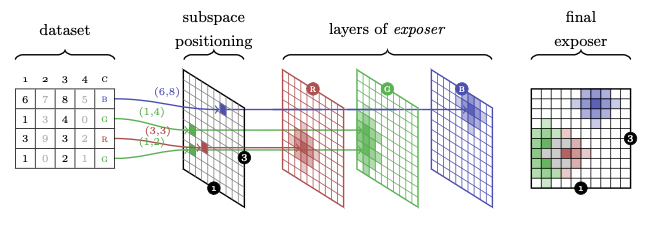
\includegraphics[width=\textwidth]{figures/exposer-projection}
	\caption{Ekspozycja czterech obiektów opisujących trzy klasy w dwuwymiarowej podprzestrzeni czterowymiarowego problemu.}\label{fig:exposer-projection}
\end{figure}

Wizualizacja procesu ekspozycji dla czterech obiektów opisujących trzy klasy w dwuwymiarowej podprzestrzeni czterowymiarowego problemu przedstawiona została na Rysunku~\ref{fig:exposer-projection}. W pierwszym kroku odbywa się tutaj pozycjonowanie podprzestrzenne, w którym każdy z obiektów zawartych w zbiorze uzyskuje nowe współrzędne w skończonej, planarnej projekcji na siatce $10\times 10$ (parametr ziarna). Ekspozer składa się z tylu warstw, ile klas zawiera się w zbiorze danych, a każda z~nich czuła jest jedynie na obiekty przynależącej do niej klasy.  

Przyjmijmy, że $\mathcal{DS}$ określa zbiór $n$ instancji, z których każda ($x_k$) reprezentowana jest przez $d$-wymiarowy wektor atrybutów oraz etykietę $i_k$ ze skończonego zbioru etykiet $\mathcal{M}$.

\begin{equation}
	\begin{array}[b]{llll}
		\mathcal{X} & \subseteq & \Re^d\\
		\mathcal{M}&=&\{1, 2, \ldots, M\}\\
		x_k & = & [x_k^{(1)}, x_k^{(2)}, \ldots, x_k^{(d)}]^{T}, & x_k \in \mathcal{X} \\
%		i_k & = & [i_1, i_2, \dots, i_n],                    & i_k \in \mathcal{M} \\
		\mathcal{DS} & = & \Big\{(x_1,i_1),(x_2,i_2),\ldots,(x_n,i_n)\Big\}
	\end{array}
\end{equation}

Różnorodność możliwych do zbudowania ekspozerów wyraża się przez zbiór $\Lambda$, zawierający ${d \choose s}$ kombinacji $\lambda_i$, gdzie $s$ stanowi wybraną wymiarowość ekspozera, w planarnym wypadku wynoszącą 2.

\begin{equation}
	\begin{array}[b]{llll}
		\Lambda   & = & \{\lambda_1, \lambda_2, \ldots, \lambda_L \}, & \vert\Lambda\vert = L= {d \choose s}                               \\
		\lambda_i & = & [l_1, l_2, \ldots, ,l_s],                     & l_j \in \{1, 2,\ldots, d\},\quad l_1\neq l_2 \neq \ldots \neq l_s,
	\end{array}
\end{equation}

Przy takich założeniach, reprezentacją ekspozera ($\mathcal{E}$) jest s-wymiarowa kostka danych:

\begin{equation}
	\begin{array}[b]{lll}
		\mathcal{E}_m & \in & G^s = \underbrace{G \times G \times \ldots \times G}_s                                                       \\
		\mathcal{E}   & =   & \{\mathcal{E}_1, \mathcal{E}_2, \ldots, \mathcal{E}_M \},
	\end{array}
\end{equation}

\noindent gdzie każda komórka adresowana przez $loc$ zawiera wektor wartości

\begin{equation}
	\begin{array}[b]{lll}
		\mathcal{E}^{(loc)} & = & [v_1, v_2, \ldots, v_M]^T       \\
		loc                 & = & [loc_1, loc_2, \ldots, loc_s]^T
	\end{array}
\end{equation}

Pojedyncza wartość jest sumą wszystkich pozytywnych różnic zadanego promienia oddziaływania $r$ z dystansem pomiędzy punktem centralnym komórki ($loc$) i każdym punktem $loc_k$ dla którego $i_k=m$. 

\vspace{-1em}\begin{equation}
	\begin{array}[b]{lll}
		\mathcal{E}_m^{(loc)} & = & \sum_{k=1}^{n}\Big[d(loc, loc_k) < r\;\wedge\; i_k = m\Big] \cdot \Big(r-d(loc,loc_k)\Big) \\
		loc_k                 & = & [ x_k^{(\lambda_1)}, x_k^{(\lambda_2)}, \ldots, x_k^{(\lambda_s)}]^T
	\end{array}
\end{equation}

Ekspozer $\mathcal{E}$, zbudowany na podprzestrzeni $\lambda$ zbioru uczącego $\mathcal{LS}$ może zostać wykorzystany do inferencji dla obiektu testowego $x_k$ ze zbioru testowego $\mathcal{TS}$ przez spróbkowanie go po projekcji do wspólnej przestrzeni

\begin{equation}
	\Psi(x_k) = \mathop{argmax}\limits_{m \in \mathcal{M}}\Big(\mathcal{E}^{(loc_k)}_m \Big).
\end{equation}

Podobnie jak w przypadku zastosowania \emph{Extreme Learning Machines} do klasyfikacji atrybutów statystycznych uzyskanych z sygnatur spektralnych, i tutaj do konstrukcji właściwego systemu rozpoznawania wykorzystywany jest nie pojedynczy, podprzestrzenny model, a zespół ekspozerów $\Pi$ zbudowany na zbiorze kombinacji $\Lambda'$ stanowiącym podzbiór wszystkich możliwych $s$-wymiarowych podprzestrzeni $\Lambda$

\begin{equation}
	\begin{array}[b]{cllll}
		\Lambda' & \subset & \Lambda, & \vert\Lambda'\vert = N, & N < L \\
		\Pi      & =       & \{\Psi_1, \Psi_2, \ldots,\Psi_N \},& \Psi : \mathcal{X} \leftarrow \mathcal{M}
	\end{array}
\end{equation}

Końcowy schemat przetwarzania stanowi trzypoziomowy zespół klasyfikatorów przedstawiony na Rysunku~\ref{fig:ece}. Jego najniższy poziom to zbiór monochromatycznych warstw, budujących drugi poziom, klasyfikatorów bazowych zespołu dla podprzestrzeni $\lambda_i$, integrowanych na ostatnim poziomie we właściwy system wieloklasyfikatorowy \emph{Exposer Classifier Ensemble} (\textsc{ece}).

\begin{figure}[!htb]
	\centering
	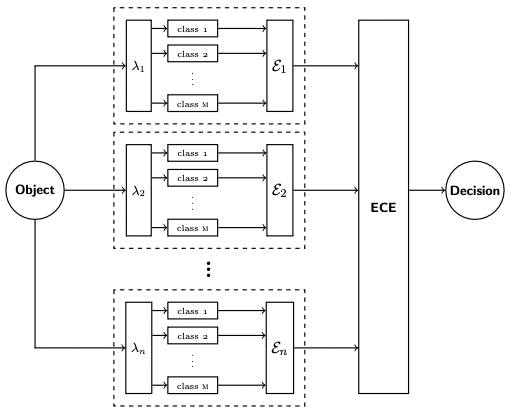
\includegraphics[width=\textwidth]{figures/ece}
	\caption{Schemat zespołu ekspozerów.}\label{fig:ece}
\end{figure}

% SKRÓĆ DWA AKAPITY PONIŻEJ I ZAPISZ TYLKO OGÓLNE WNIOSKI
Zaproponowana w pracy metoda została poddana ewaluacji z wykorzystaniem pakietu \emph{Weles}\sidenote{Weles -- Collection of various pattern recognition methods and experimental tools made by ML Group of Wrocław University of Science and Technology. --- \url{https://github.com/w4k2/weles}} opracowanego w ramach bieżących prac \emph{Zespołu Uczenia Maszynowego, Katedry Systemów i Sieci Komputerowych}. Jak można zauważyć dzięki przeprowadzonej analizie, \textsc{ece} często osiąga szczyt swojej efektywności przy relatywnie niskich wartościach hiperparametrów, jakkolwiek trudniejsze, wielowymiarowe i silnie niezbalansowane problemy przesuwają tę granicę wykazując, że wzrost próbkowania może mieć pozytywny wpływ na jakość klasyfikacji. W większości przypadków proponowane rozwiązanie osiąga rezultaty istotnie lepsze od pozostałych modeli bazowych, w żadnym przypadku nie okazując się najsłabszą metodą w stawce.

Algorytm \textsc{ece} wykorzystując informację o rozkładzie klas wykazuje przewagi typowe z klasyfikatorów bayesowskich, osiągając najlepsze rezultaty dla danych niezbalansowanych. Dodatkowo, dzięki strategii próbkowania podprzestrzennego pozostaje on w dużym stopniu odporny na zjawisko klątwy wielowymiarowości, ponieważ obiekty interpretowane są w nim jedynie w niskowymiarowych reprezentacjach. Łącząc te przewagi z regułą inferencyjną typową dla klasyfikatorów minimalnoodległościowych okazuje się on stabilnym rozwiązaniem dla trudnych przypadków danych jednocześnie niezbalansowanych i wielowymiarowych.  

\subsection*{II -- Algorytmy przetwarzania danych niezbalansowanych}

\marginnote{\scalebox{.6}{\large
	\def\imbcircle{(-210:2) circle (2.725cm)}
	\def\dscircle{(-330:2) circle (2.725cm)}
	\def\mdcircle{(-90:2) circle (2.725cm)}

	\begin{tikzpicture}
      	
      	\node[fill=black,rotate=0, text width=5.25cm, text height=2.9cm] at (90:-.5) {};
		\node[color=white,fill=black,rotate=0,rounded corners=.25cm, text width=5.25cm, align=center] at (90:1.25) {\bfseries \textsc{dane niezbalansowane}};
      	
      	\draw[fill=white] \mdcircle;
      	\draw[ultra thick] \mdcircle;
      	
      	\node at (-90:.5) {[C8]};    
      	\node at (-90:1.25) {[C6]};          	
      	    	   
      	\node at (-90:2) {\color{black!50}\emph{[C2]}};   
      	\node at (-90:2.75) {\color{black!50}\emph{[C3]}};   
      	\node at (-90:3.5) {\color{black!50}\emph{[C4]}};   
      	\node at (-90:4.25) {\color{black!50}\emph{[C9]}};
	\end{tikzpicture}}}

Drugim istotnym wątkiem moich prac realizowanych po uzyskaniu stopnia naukowego doktora jest przetwarzanie danych niezbalansowanych. Elementy tego rodzaju przetwarzania obecne są już w pracach przedstawionych we wcześniejszej sekcji, ale wyodrębniłem też w badaniach jednoznaczny wątek traktujący ten problem jako podstawowe zagadnienie analiz.

Po prawej stronie diagram zaznaczający opisywane w ramach wątku przetwarzania danych niezbalansowanych, wliczający prace opisane w~innych wątkach dominujących.
\vspace{1em}

{
\color{red}
\noindent\begin{tabular}{p{\textwidth}}
	\toprule &
\end{tabular}\vspace{-1em}
}
\noindent Przykładem takiego podejścia jest praca \citeC[-2.25em]{C6}, proponująca hybrydowe rozwiązanie łączące dywersyfikację podprzestrzenną z nadpróbkowywaniem syntetycznym. Strategia taka pozwala na budowę zespołu klasyfikatorów integrującego oversampling w procedurze konstrukcji systemu wieloklasyfikatorowego w miejsce stosowanego standardowo potoku rozłącznych akcji \emph{preprocessing $\rightarrow$ modelowanie}. W typowym podejściu do konstrukcji tego rodzaju systemów, faza preprocessingu nie jest specyficzna dla dywersyfikowanych modeli, a dokonuje się przed uróżnorodnieniem puli.

Konstrukcja dowolnego zespołu klasyfikatorów wiąże się z~dwiema podstawowymi trudnościami. Pierwszą jest zapewnienie różnorodnej puli klasyfikatorów pozwalającej na realizację niezależnych predykcji. Możemy osiągnąć to przez wykorzystywanie różnych modeli -- w~ramach dywersyfikacji heterogenicznej -- lub też przez modyfikację zestawu danych treningowych -- przy bardziej czytelnej w integracji dywersyfikacji homogenicznej. Proponowana metoda wykorzystuje to drugie podejście, w~którym każdy klasyfikator jest trenowany na losowej podprzestrzeni zbioru uczącego. Redukcja przestrzenności problemu, poza zapewnieniem różnorodności, stanowi również czynnik różnicujący efekt nadpróbkowywania. Standardowe metody syntetycznego oversamplingu, takie jak \textsc{smote}~\citeZ{Z25} czy \textsc{adasyn}, opierają się najczęściej na ocenie podobieństwa wzorców określanego przez metryki dystansowe, którego struktura zmienia się wraz z~każdą modyfikacją zbioru uczącego inną niż losowy obrót przestrzeni problemu~\citeZ{Z24}.

Drugą trudnością typową dla projektowania zespołu klasyfikatorów jest zapewnienie odpowiedniej reguły decyzyjnej, integrującej predykcje modeli dostępnych w puli. Najbardziej obiecującym rozwiązaniem w tym wypadku -- pozwalającym na przekroczenie ograniczenia abstrakcyjnej reguły decyzyjnej Wyroczni\footnote{Wyroczna -- w zakresie uczenia zespołowego -- stanowi abstrakcyjną regułę decyzyjną o nieuprawnionym dostępie do etykiet, podejmującą słuszną decyzję zawsze, kiedy skłania się ku niej co najmniej jeden z klasyfikatorów w puli.} stawianego regułom opartym na głosowaniu większościowym -- jest akumulacja wsparć klasyfikatorów bazowych. Należy jednak pamiętać, że wymaga ona wykorzystania wyłącznie klasyfikatorów udostępniających funkcję decyzyjną, klasyfikatorów problabilistycznych lub modeli o interpretacji probabilistycznej. Regułę taką można dodatkowo rozbudować przez wprowadzenie ważenia, które w rozważanym przypadku oparte było na wyznaczonej przez metrykę $F_1$ jakości osiąganej przez każdy z modeli wchodzących w skład puli.

Pełen schemat przetwarzania zaproponowanej metody przedstawiony został na Rysunku~\ref{fig:hais}. Zgodnie z przedstawioną procedurą, dostępny zbiór uczący dzielony jest na podzbiory jego atrybutów, a następnie obiekty klasy mniejszościowej każdej zredukowanej tak reprezentacji są syntetyzowane do poziomu zbalansowania przez algorytm \textsc{smote}, aby na każdej lokalnie zrównoważonej reprezentacji zbudować nowy model. Tak skonstruowana pula klasyfikatorów integrowana jest później przez akumulację wsparć ważoną przez wartość metryki $F_1$ osiągniętej na pełnym zbiorze uczącym.

\begin{figure}[h]
	\centering
	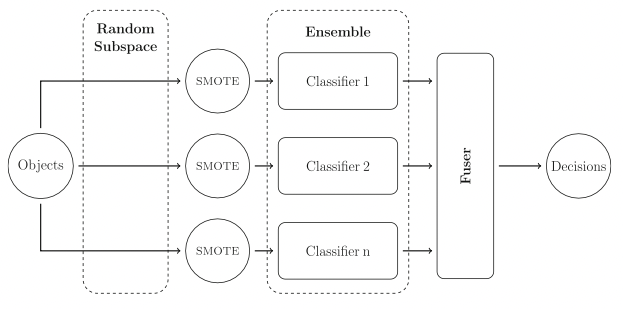
\includegraphics[width=\textwidth]{figures/hais}
	\caption{Schemat architektury zespołu klasyfikatorów zaproponowanego w pracy \emph{Combining Random Subspace Approach with \textsc{smote} Oversampling for Imbalanced Data Classification}.}\label{fig:hais}
\end{figure}

Zaproponowana metoda została poddana ewaluacji eksperymentalnej z wykorzystaniem 30 zbiorów danych o różnej, wysokiej skali niezbalansowania, dostępnych w repozytorium \textsc{keel}\sidenote[][]{Knowledge Extraction Evolutionary Learning -- dataset repository\\\noindent\url{https://sci2s.ugr.es/keel/datasets}}. W ramach ewaluacji przetestowano efektywność rozwiązania dla trzech klasyfikatorów o~interpretacji probabilistycznej: \emph{Gaussian Naive Bayes}, \emph{Logistic Regression} i~\emph{Support Vector Machine}. Analiza miała na celu porównanie ze sobą sześciu podejść:

\begin{itemize}
	\item uczenia na oryginalnym zbiorze,
	\item globalnego oversamplingu \textsc{smote},
	\item dywersyfikacji przez losowe podprzestrzenie,
	\item połączenia dywersyfikacji przez losowe podprzestrzenie z lokalnym oversamplingiem \textsc{smote},
	\item ważonego przez metrykę \emph{F1-score} zespołu o surowej dywersyfikacji przez losowe podprzestrzenie,
	\item ważonego przez metrykę \emph{F1-score} zespołu łączącego dywersyfikację przez losowe podprzestrzenie z lokalnym oversamplingiem \textsc{smote}.
\end{itemize}

Analiza uzyskanych wyników pozwala zaobserwować, że niezależnie od wykorzystanego klasyfikatora bazowego, użycie globalnego oversamplingu \textsc{smote} wpływa pozytywnie na jakość rozpoznawania, z reguły ulepszając model bazowy. 

Patrząc na drugi istotny czynnik przetwarzania, wykorzystanie jedynie dywersyfikacji przez losowe podprzestrzenie, przy warunkach wysokiego niezbalansowania, prowadzi do bardzo niskich rezultatów, pogarszających nawet jakość klasyfikatora bazowego. Wprowadzenie ważenia zespołu ulepsza taki model, prowadząc do rezultatów lepszych niż bazowy, ale nadal gorszych niż globalny \textsc{smote}.

Wykorzystanie obydwu tych strategii, w formie zespołu z lokalnym nadpróbkowywaniem, prowadzi do rezultatów odrobinę lepszych niż globalny \textsc{smote}, co może sugerować, że pozytywny wpływ obu tych czynników jest niezależny od siebie i potencjalnie może okazać się komplementarny. Potwierdzają to rezultaty osiągane przez pełną propozycję rozwiązania, ważony zespół łączący dywersyfikację przez losowe podprzestrzenie z lokalnym oversamplingiem, którego jakość jest jednoznacznie najlepsza w puli analizowanych przykładów.

Praca uprawdopodabnia stwierdzenie, że wspólne wykorzystanie metod balansowania i dywersyfikacji, przy kontroli wpływu każdej podprzestrzeni na finalną predykcję przez ważenie zgodne z efektywnością w problemie niezbalansowanym, może prowadzić do zbliżenia się do optymalnego rozmieszczenia obiektów uczących w przestrzeni problemu i tym samym prowadzić do budowy modeli o wysokiej zdolności dyskryminacyjnej.\vspace{1em}

\newpage
{
\color{red}
\noindent\begin{tabular}{p{\textwidth}}
	\toprule &
\end{tabular}\vspace{-1em}
}
\noindent Wykorzystanie metod resamplingu w konstrukcji systemów rozpoznawania dla danych niezbalansowanych nierozerwalnie niesie ze sobą ryzyko utraty informacji o potencjalnie istotnych obiektach klasy większościowej. Możliwa jest jednak mitygacja tego problemu, przez odpowiednie wykorzystanie podejścia zespołowego, które pozwoli na pełne wykorzystanie dostępnych danych bez konieczności syntetyzacji nowych wzorców lub redukcji obiektów istniejących. Propozycję algorytmu tego rodzaju przedstawiłem w pracy \citeC[-12em]{C8}.

Metoda ta dedykowana jest jedynie problemom binarnym o wysokim stopniu niezbalansowania, gdzie \emph{imbalanced ratio} (\textsc{ir}) wynosi 1:9 i~więcej. Złożone metody resamplingu, takie jak \textsc{smote} czy \textsc{adasyn}, pomimo wysokiej efektywności w~wielu niezbalansowanych problemach rozpoznawania, nie odnajdują swojego zastosowania w~scenariuszach skrajnych, gdzie klasa mniejszościowa reprezentowana jest jedynie przez kilka przykładów pośród których nie jest możliwa analiza sąsiedztwa pozwalająca na syntetyzację nowego obiektu. Teoretycznie możliwe jest w~takiej sytuacji zastosowanie undersamplingu, ale jak pokazują badania, rozwiązania takie w sytuacjach silnego niezbalansowania nie pozwalają na uzyskanie stabilnego systemu rozpoznawania.

Popularnym rozwiązaniem w takiej sytuacji jest wykorzystanie standardowych zespołów opartych na \emph{Baggingu} lub \emph{Boostingu} -- opartych na losowym próbkowaniu ze zwracaniem, które pozwalają na rozbicie dużego problemu w~serię mniejszych. W~pracy proponuję prostą obliczeniowo metodę, która również dokonuje rozbicia problemu rozpoznawania, zapewniając jednak obecność wszystkich obiektów dostępnych w~zbiorze uczącym, eliminując również ryzyko nakładania się klas.

Model \emph{Undersampled Majority Class Ensemble} (\textsc{umce}) buduje się zgodnie z następującymi krokami:

\begin{fullwidth}\vspace{2em}
\hspace{1em}\begin{minipage}{30em}
\begin{itemize}
	\item[1.] Podziel $\mathcal{DS}$ na zbiór mniejszościowy $MinC$ i większościowy $MajC$.
	\item[2.] Wyznacz współczynnik niezbalansowania $IR$ jako proporcję liczności zbiorów $MinC$ i $MajC$.
	\item[3.] Wyznacz współczynnik $k$ jako najbliższe całkowite zaokrąglenie $IR$.
	\item[4.] Zrealizuj k-foldowy podział zbioru $MajC$, aby wytworzyć zbiór podzbiorów $MajC_1, MajC_2, \ldots, MajC_k$.
	\item[5.] Dla każdego $i$ w zakresie do $k$:
	\begin{itemize}
		\item[6.] Złącz zbiory $MajC_i$ i $MinC$ w zbalansowany zbiór $\mathcal{TS}_i$.
		\item[7.] Zbuduj model $\Psi_i$ na podstawie przykładów $\mathcal{TS}_i$ i dodaj go do zespołu.
	\end{itemize} 
\end{itemize}
\end{minipage}\vspace{2em}
\end{fullwidth}

Opcjonalnym elementem przetwarzania jest uzupełnienie puli modeli o dodatkowy klasyfikator zbudowany z wykorzystaniem typowego zastosowania algorytmu \textsc{smote}. Został on włączony do metody aby umożliwić weryfikację różnic w zyskach z obu strategii, podobnie jak miało to miejsce w poprzednio opisanej pracy.

Klasycznie już, istotnym elementem metody zespołowej jest również reguła integracji. W wypadku algorytmu \textsc{umce} zdecydowałem się odejść od prostych paradygmatów fuzji wsparć, rozwijając strategię podstawową (\textsc{reg}) i ważoną proporcjonalnie do jakości (\textsc{wei}) o trzy dodatkowe propozycje:

\begin{itemize}
	\item[\bfseries\textsc{nor}] \textbf{Normalizowana przedziałowo akumulacja ważona} -- pozwalająca na istotne wzmocnienie najlepszego klasyfikatora w puli i całkowitą redukcję wpływu klasyfikatora najsłabszego.
	\item[\bfseries\textsc{con}] \textbf{Dynamiczna akumulacja wsparć}. Aby zapewnić lepsze wykorzystanie klasyfikatorów o większej "pewności" decyzji względem danego obiektu, decyzja dla każdego wzorca ważona jest przez bezwzględną różnicę pomiędzy wsparciami, która na potrzeby badań została nazwana \emph{kontrastem}. Ilustracją tego podejścia jest Rysunek~\ref{fig:contrast}, na osiach X prezentujący próbki, a na osiach Y -- klasyfikatory dostępne w puli. Białe punkty pokazują kontrast 1, a więc decyzję pewną, podczas gdy czarne powiązane są z kontrastem 0, a więc absolutnym brakiem pewności, czyli wzorcem leżącym bezpośrednio na granicy decyzyjnej.
	\item[\bfseries\textsc{nci}] \textbf{Akumulacja wsparć ważona przez iloczyn \textsc{nor} i \textsc{con}}.
\end{itemize}

\begin{figure}[!htb]
	\vspace{-1em}\centering
	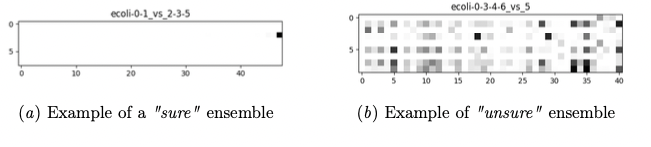
\includegraphics[width=\textwidth]{figures/contrast}
	\caption{Ilustracja rozkładu \emph{kontrastu} w zespołach klasyfikatorów zbudowanych na dwóch zbiorach danych.}\label{fig:contrast}
	\vspace{-2em}
\end{figure} 

Należy pamiętać, że zaproponowana metoda budowy zespołu uzależnia jego wielkość od poziomu niezbalansowania, co dla danych bardzo silnie niezbalansowanych (przykładowo o IR 1:100) prowadzić będzie do konstrukcji bardzo dużego modelu hybrydowego. W związku z tym, zaproponowana została również metoda przycinania zespołu klasyfikatorów.

Typowe metody przycinania zespołów działają w trybie statycznym, analizując jakość modeli członkowskich i wycinając pulę klasyfikatorów o najniższym potencjale dyskryminacyjnym. W pracy zaproponowałem jednak metodę przycinania dynamicznego, dostosowującego skład zespołu do zbioru testowego. Zespół, otrzymując na wejściu zbiór testowy, generuje wektory wsparć ($s_i$) dla każdego klasyfikowanego obiektu, co pozwala zinterpretować wsparcia dla danej klasy z danego klasyfikatora jako zmienne losowe możliwe do analizy wzajemnej zależności statystycznej. W propozycji, wykorzystując test rankingowy, dokonuję klasteryzacji puli $k$ modeli do $n$ grup ($n \leq k$) celem uśrednienia wsparć i wag w obrębie każdej grupy przed końcową integracją. 

Pełen schemat organizacji metody \textsc{umce} z rozbiciem na blok indukcyjny i predykcyjny przedstawiony został na Rysunku~\ref{fig:umce}.

\begin{figure}[!htb]
	\centering
	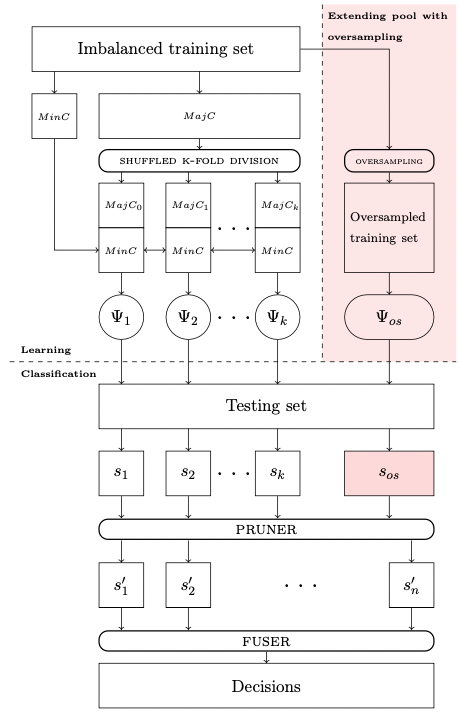
\includegraphics[width=.9\textwidth]{figures/umce}
	\vspace{-1em}
	\caption{Schemat organizacji metody \emph{Undersampled Majority Class Ensemble}.}\label{fig:umce}
\end{figure}

Ewaluacja eksperymentalna metody \textsc{umce} została zrealizowana na 40 binarnych problemach klasyfikacji o \textsc{ir} większym niż 1:9. Aby umożliwić właściwe porównanie z metodami referencyjnymi zastosowano klasyczną, pięciofoldową walidację krzyżową, a w ocenie jakości modeli zastosowana została metryka zbalansowanej dokładności.

Metoda bazowa osiągnęła przewagę nad konkurencją jedynie w~trzech przypadkach, podczas gdy standardowe metody over- i~undersamplingu okazały się najlepsze w~nie więcej niż dwóch przypadkach, niezależnie od zastosowanego klasyfikatora bazowego. Jednak, zarówno rozszerzenie puli klasyfikatorów \textsc{umce} o~model wykorzystujący \textsc{smote}, jak i~zaproponowana metoda pruningu oraz mieszana metoda ważenia \textsc{nci} prowadzą do jednoznacznie najlepszych rezultatów w~porównaniu. Należy podkreślić skuteczność metody \textsc{umce} tym bardziej, że nawet najprostsza forma jej architektury, pozbawiona przycinania i~ważenia zespołu, osiąga wyniki istotnie lepsze niż metody \emph{state-of-the-art} dziedziny.

\subsection*{III -- Algorytmy przetwarzania strumieni danych}

\marginnote{\scalebox{.6}{\large
	\def\imbcircle{(-210:2) circle (2.725cm)}
	\def\dscircle{(-330:2) circle (2.725cm)}
	\def\mdcircle{(-90:2) circle (2.725cm)}

	\begin{tikzpicture}
      	
      	\node[fill=black,rotate=0, text width=5.25cm, text height=2.9cm] at (90:-.5) {};
		\node[color=white,fill=black,rotate=0,rounded corners=.25cm, text width=5.25cm, align=center] at (90:1.25) {\bfseries \textsc{strumienie danych}};
      	
      	\draw[fill=white] \mdcircle;
      	\draw[ultra thick] \mdcircle;
      	
      	% 10 9 11 
      	% MD
      	\node at (-90:0) {[C7]};
      	\node at (-90:.75) {[C4]};    
      	\node at (-90:1.5) {[C3]};    
      	\node at (-90:2.25) {[C5]};    
      	\node at (-90:3) {[C2]};    
      	\node at (-90:3.75) {[C1]};
	\end{tikzpicture}}}

Po prawej stronie diagram zaznaczający opisywane w ramach wątku przetwarzania strumieni danych, wliczający prace opisane w innych wątkach dominujących.

Istnieje wyraźne podobieństwo pomiędzy wsadowym podejściem do predykcji, wykorzystywanym w procedurze przycinania algorytmu \textsc{umce}, a typowymi strategiami przetwarzania strumieni danych, które swoją ewaluację opierają na protokole \emph{Test-Then-Train}. Środowisko tego rodzaju pozwala nie tylko na wnioskowanie względem pojedynczego predykowanego obiektu, ale też udostępnia kontekst, w którym obiekt ten pojawia się w toku przetwarzania. Rozwiązania takie stanowią trzeci, kluczowy wątek prac realizowanych przeze mnie w ramach omawianego cyklu publikacji podejmującego tematykę klasyfikacji danych trudnych.\vspace{1em}

{
\color{red}
\noindent\begin{tabular}{p{\textwidth}}
	\toprule &
\end{tabular}\vspace{-1em}
}
\noindent Pierwszą omawianą pracą z tej kategorii jest artykuł~\citeC[-2.25em]{C7}. Podejmuje on tematykę wykorzystania efektu \emph{catastrophic forgetting} -- typowego dla sieci neuronowych -- w adaptacyjnej klasyfikacji strumieni danych podatnych na zjawisko dryfu koncepcji przy redukcji zaangażowania ekspertów w uzyskiwaniu oznaczenia danych. 

Strategie uczenia się przy ograniczonej etykietyzacji dla problemów stacjonarnych, często opierają się na klasteryzacji dostępnych obiektów pozwalającej na transdukcyjną identyfikację prototypów, które po oznaczeniu przez eksperta stanowią później przypadki reprezentatywne dla wydzielonych podzbiorów zbioru uczącego. W wypadku uczenia inkrementalnego i strumieniowego częściej jednak wykorzystywany jest paradygmat uczenia aktywnego, w którym pewna wiedza -- zakumulowana już przez przyrostowy model -- może być wykorzystywana do identyfikacji tzw. przypadków trudnych w obrębie nowego, nieoznaczonego jeszcze wsadu.

Podstawowym zagadnieniem poruszanym w pracy jest istotna redukcja kosztów konstrukcji systemu rozpoznawania w środowisku strumieniowym przy jednoczesnym zachowaniu efektywności, którą uzyskałby przy pełnym dostępie do etykiet. W wielu zadaniach praktycznych niemożliwe jest pozyskanie odpowiedniego zbioru etykiet w racjonalnym czasie, a jednocześnie niemal zawsze wymaga ona wykorzystania czynnika ludzkiego, który jest zarówno kosztowny, jak i omylny -- szczególnie jeżeli dotyczy oznaczania danych masowych i napływających z~wysoką częstotliwością. Sprawia to, że projektowanie metod klasyfikacji, które zdolne są do budowy rzetelnych systemów rozpoznawania przy jedynie częściowej etykietyzacji jest jednocześnie dużym wyzwaniem, jak i~nadal bardzo pożądanym celem badań. W~ramach pracy proponowany jest hybrydowy model uczenia aktywnego, łączący podejścia typowe dla uczenia online wraz ze strategiami okna przesuwnego.

Przyjmujemy, że jeżeli decyzja dla zadanego obiektu wynika z wysokiej wartości wsparcia, leży on daleko od granicy decyzyjnej, a więc wykorzystanie go w budowie modelu nie będzie mieć istotnego wpływu na zmianę estymowanego prawdopodobieństwa \emph{a posteriori}. W wypadku modeli interpretowanych probabilistycznie wysoka wartość funkcji wsparcia oznacza też niewielkie prawdopodobieństwo błędu klasyfikacji. Stąd znacznie bardziej~"\emph{interesujące}"~dla procedury modelowania są przypadki trudne, o niepewnej decyzji -- rozumianej jako niewielka różnica pomiędzy wsparciami dla kategorii konkurujących między sobą o decyzję eksperta. 

Aby sformalizować to założenie, zaproponowana została funkcja $RSFD$ (\emph{Relative Support Function Difference}), mierząca średnią różnicę pomiędzy największym prawdopodobieństwem i każdym z pozostałych elementów wektora wsparć dla zadanej obserwacji $x$

\begin{equation}
	RSFD(x) = \frac{\sum_{i=1}^{M}[ \max_{k\in\mathcal{M}}(F_k(x)) - F_i(x)]}{M-1},
\end{equation}

\noindent gdzie $Fi(x)$ to wartość wsparcia klasyfikatora $i$ dla obiektu $x$. 

Graficzna interpretacja funkcji $RSFD$ dla przypadku dwu- i trzyklasowego zaprezentowana jest również na Rysunku~\ref{fig:neuro1}. Barwy na ilustracji prezentują wsparcia dla klas, a spadek wartości w podglądzie monochromatycznym -- trudność przypadków objętych obszarem.

\begin{figure}[!htb]
	\centering
	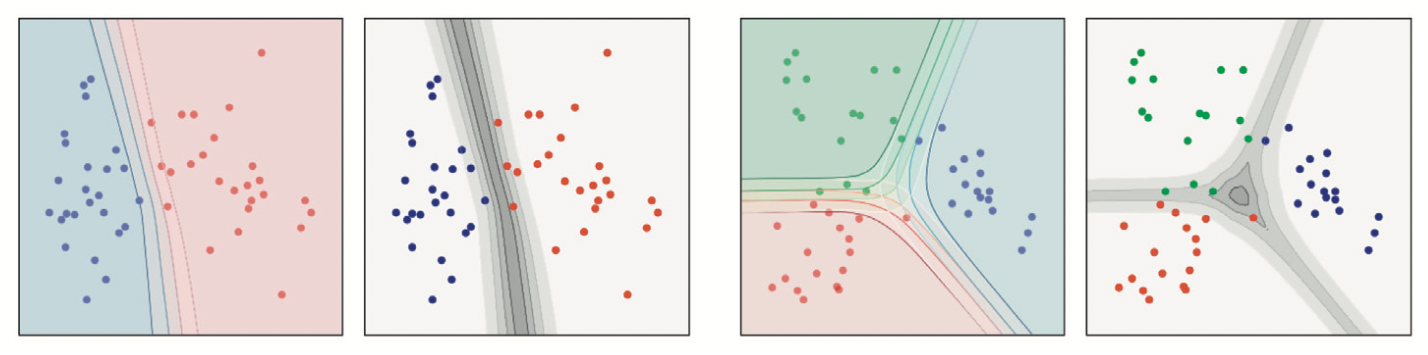
\includegraphics[width=\textwidth]{figures/neuro1}
	\caption{Przykład rozkładu wsparć i wartości funkcji RSFD dla dwuwymiarowych zbiorów o dwóch i trzech klasach problemu.}\label{fig:neuro1}
\end{figure}

Klasycznie, podejście takie wykorzystywane jest w~\emph{klasyfikacji z~opcją odrzucenia} (ang. \emph{classification with reject option}\citeZ{Z26}), gdzie decyzje podejmowane są jedynie dla przypadków względem których klasyfikator jest w stanie podjąć dostatecznie pewną decyzję. W proponowanym przetwarzaniu zasada ta jest jednak odwracana i~fakt \emph{odrzucenia} danego obiektu jest powiązany z~identyfikacją go jako obserwacji interesującej i~skierowaniem do oznaczenia przez eksperta. Celem umożliwienia kontroli tego procesu wprowadzone zostały dwa hiperparametry metody:

\begin{itemize}
	\item \emph{próg} -- wprowadzający wartość graniczną średniej różnicy wsparć, poniżej której obiekt uznawany jest za interesujący,
	\item \emph{budżet} -- określający jaki największy odsetek wsadu uczącego może zostać skierowany do etykietyzacji.
\end{itemize}

Całość zrealizowanej ewaluacji eksperymentalnej, jak w większości wchodzących w skład cyklu prac podejmujących przetwarzanie strumieniowe, wykonana została w oparciu o model \emph{Multilayer Perceptron}. Efekty przeprowadzonej analizy pozwoliły na uprawdopodobnienie hipotezy o możliwości znaczącej redukcji kosztu etykietyzacji przy jednoczesnym zachowaniu zdolności dyskryminacyjnej modeli strumieniowych. Wstępne badania wykazały, że proste podejście budżetowe, pomijające całkowicie aspekt aktywnego doboru wzorców do etykietyzacji, liniowo degraduje krzywą uczącą, istotnie wydłużając czas konwergencji modelu. Wykorzystanie tej samej, lub nawet niższej liczby wzorców, dobranych jednak zgodnie z sugestiami dotychczasowego modelu, niweluje ten efekt, często pozwalając nawet na eliminację zapotrzebowania na eksperta w stabilnej fazie koncepcji. 

Co szczególnie interesujące i~możliwe do zaobserwowania w~eksperymentach rozszerzonych, osiągany efekt w~niektórych przypadkach pozwala nie tylko na zachowanie zdolności dyskryminacyjnych modelu o pełnej etykietyzacji, ale też wykazuje zdolność do eliminacji obiektów o~negatywnym wpływie na model i~prowadzi do osiągnięcia wcześniejszej zbieżności sieci neuronowej. Pokazuje to, że dziedzina przetwarzania strumieni danych nadal jest obszarem o~dużym potencjale rozwijania badań, w~szczególności tych dotyczących budowy modeli neuronowych w~środowiskach o~zmiennych koncepcjach.

Najpowszechniej podejmowanym w literaturze obszarem badań z~zakresu strumieni danych jest analiza zdolności systemów uczących się do adaptacji do zmian w~prawdopodobieństwie a posteriori problemu, a~więc do dryfu koncepcji. Interesującym badawczo obszarem jest jednak również punkt styku pomiędzy tą tematyką, a~problemem niezbalansowania danych, zdefiniowanym jako jeden z~trzech głównych obszarów tematycznych prezentowanego cyklu.\vspace{1em}

{
\color{red}
\noindent\begin{tabular}{p{\textwidth}}
	\toprule &
\end{tabular}\vspace{-1em}
}
\noindent Analizując to zagadnienie, w artykule~\citeC[-2.25em]{C4} wykazałem, że możliwe jest uwzględnienie estymowanego prawdopodobieństwa a priori strumienia danych o stałym stopniu niezbalansowania w istotnym statystycznie polepszeniu mocy generalizacyjnej modeli rozpoznawania. Podstawą analizy była weryfikacja potencjału przetwarzania końcowego (\emph{postprocessingu}) w ulepszaniu modelu klasyfikacji strumieni niezbalansowanych statycznie bez ingerowania w procedurę budowy modelu.

W ramach pracy zaproponowana została metoda \emph{Prior Imbalance Compensation} (\textsc{pic}), generująca stosunkowo minimalny narzut obliczeniowy i zaprojektowana dla strumieni, w których nowe instancje pojawiają się z wysoką częstotliwością i w dużych ilościach lub dla przypadków o bardzo dużej skali niezbalansowania (w której odsetek klasy mniejszościowej stanowi mniej niż 5\% ogółu dostępnych danych). Tak silne zaburzenie proporcji pomiędzy klasami, jak wskazane zostało już w opisie metody \textsc{umce}, uniemożliwia syntetyzację wzorców metodą \textsc{smote}, a~więc wymaga alternatywnych strategii przetwarzania.

Algorytm \textsc{pic}, na podstawie dotychczas etykietowanych przypadków, przy najbardziej typowym dla literatury założeniu o stabilności niezbalansowania, z rosnącą precyzją estymuje prawdopodobieństwa \emph{a priori} przetwarzanego problemu. Estymacja ta nie jest wykorzystywana przy budowie modelu, która odbywa się w klasyczny sposób, ale stanowi podstawę dla korekty uwzględnianej przy predykcji wsadowej. Jest ona możliwa do realizacji dla dowolnego modelu o interpretacji probabilistycznej lub o ciągłych funkcjach decyzyjnych, a więc przetestowana została w oparciu o klasyfikatory \emph{Naive Bayes}, \emph{k-Nearest Neighbors}, \emph{Random Trees} oraz \emph{Support Vector Machine}.

Zrealizowana ewaluacja eksperymentalna oceniała efektywność klasyfikacji strumieni niezbalansowanych (przetestowano problemy od zbalansowanych do niezbalansowanych w skali 1:20) zgodnie ze wskazaniami metryk zbalansowanej dokładności i \emph{F1-score}. Kompensacja aprioryczna \textsc{pic} pozwoliła na uzyskanie istotnego statystycznie polepszenia zbalansowanej dokładności klasyfikacji z niewielkim spadkiem metryki \emph{F1-score} w każdym z testowanych scenariuszy. Szczególnie wyraźne jest to dla modeli opartych o \emph{Support Vector Machine}.

%\begin{table}[!htb]
%	\centering
%	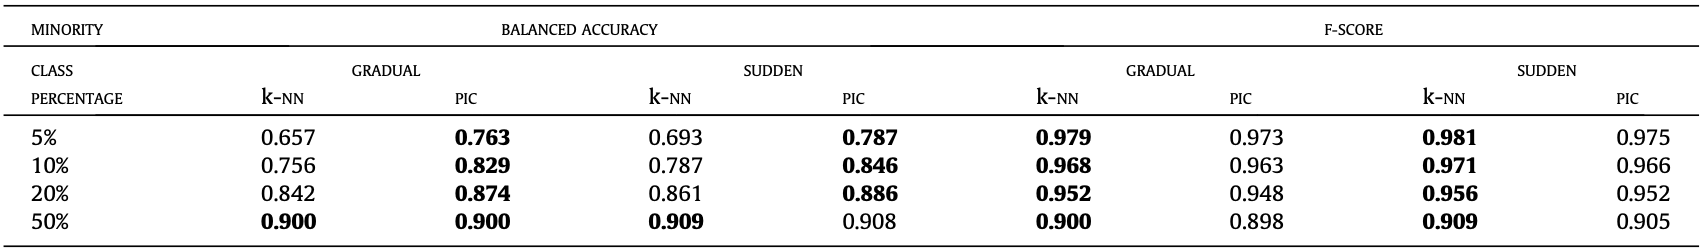
\includegraphics[width=\textwidth]{figures/pic}
%	\caption{Zbalansowana dokładność i miara F-score dla strumieni niezbalansowanych o rosnącym współczynniki niezbalansowania.}\label{tab:pic}
%\end{table}

Korekta aprioryczna ma też pewien wpływ na klasyfikację strumieni zbalansowanych, ale stanowi ona wtedy tylko niewielkie zaburzenie w~jakości. Wraz ze zwiększaniem się skali niezbalansowania, przy zachowaniu tych samych analizowanych koncepcji, widać wyraźną degenerację modeli bazowych w~domyślnej interpretacji predykcji przy jednoczesnym zachowaniu wysokiej sprawności przy zastosowaniu \textsc{pic}. Należy zaznaczyć, że w~obu przypadkach wykorzystywany jest dokładnie ten sam model, poddany jednak zmienionej interpretacji funkcji decyzyjnej.

Zbliżone obserwacje zostały dokonane zarówno na dryfach gradualnych, jak i~nagłych. Algorytm \textsc{pic} jest zdolny do ulepszenia jakości rozpoznawania dla każdego z~rozważanych modeli klasyfikacji, ale największą odporność na niezbalansowania uzyskują dzięki niemu \emph{Support Vector Machine}.\vspace{1em}

{
\color{red}
\noindent\begin{tabular}{p{\textwidth}}
	\toprule &
\end{tabular}\vspace{-1em}
}
\noindent Rozszerzone badania nad potencjałem metody \textsc{pic} pozwoliły na wstępną identyfikację nowego obszaru badawczego w zakresie przetwarzania niezbalansowanych strumieni danych, które pogłębiłem w dwóch kolejnych publikacjach prezentowanych w ramach konferencji \emph{IEEE World Congress on Computational Intelligence 2021'}~\citeC[-8em]{C3} i \emph{2022'}~\citeM[.5em]{Kom22}, z których pierwsza -- z racji na istotne rozwinięcie tej koncepcji -- włączona została do opisywanego cyklu.

W pracy rozwijana jest analiza dotycząca przetwarzania niezbalansowanych strumieni danych z uwzględnieniem potencjalnej dynamiki tych zmian. Wraz ze współautorami proponujemy tam taksonomię zjawisk niezbalansowania strumieni danych, wydzielającą następujące kategorie:

\begin{itemize}
	\item[\textsc{bs}] \textbf{Strumienie zbalansowane (\emph{balanced streams})}, gdzie globalne prawdopodobieństwo \emph{a priori} i każde z prawdopodobieństw lokalnych jest proporcjonalne i wzajemnie zależne.
	\item[\textsc{sis}] \textbf{Strumienie niezbalansowane statyczne (\emph{statically imbalanced streams})}, gdzie globalne prawdopodobieństwo \emph{a priori} i prawdopodobieństwa dla każdego kolejnego okna sąsiadujących obiektów jest nieproporcjonalne, ale wzajemnie zależne.
	\item[\textsc{dis}] \textbf{Strumienie niezbalansowane dynamicznie (\emph{dynamically imbalanced streams})}, wśród których można wydzielić dwie kategorie:
	\begin{itemize}
		\item[\textsc{cdis}] \textbf{Strumienie niezbalansowane dynamicznie w sposób ciągły (\emph{continous dynamically imbalanced streams})}, gdzie globalne prawdopodobieństwo \emph{a priori} może różnić się od prawdopodobieństwa dla każdego kolejnego okna sąsiadujących obiektów, które nie są wzajemnie zależne, ale zmieniają się w sposób ciągły, umożliwiając obserwację trendów zmian.
		\item[\textsc{ddis}] \textbf{Strumienie niezbalansowane dynamicznie w sposób dyskretny (\emph{discrete dynamically imbalanced streams})}, gdzie globalne prawdopodobieństwo \emph{a priori} może różnić się od prawdopodobieństwa dla każdego kolejnego okna sąsiadujących obiektów, które nie są wzajemnie zależne i zmieniają się dyskretnie, uniemożliwiając obserwację trendów zmian. 
	\end{itemize}
\end{itemize}

Przykładowe przebiegi prawdopodobieństwa wystąpienia klasy mniejszościowej dla przyjętej taksonomii zaprezentowane są na Rysunku~\ref{fig:stream-taxonomy}. Jak można zauważyć, klasyczny przypadek strumienia niezbalansowanego, typowy dla literatury (\textsc{sis}) charakteryzuje się stabilną proporcją o niewielkiej wariancji na całym przebiegu przetwarzania. Strumień niezbalansowany dynamicznie w sposób dyskretny (\textsc{ddis}) również wykazuje pewną wartość oczekiwaną niezbalansowania, ale wariancja estymacji prawdopodobieństwa jest już w nim na tyle duża, że może mieć istotny wpływ na jakość modelu. Strumień niezbalansowany dynamicznie w sposób ciągły (\textsc{cdis}) wykazuje charakter pośredni pomiędzy \textsc{sis} i \textsc{ddis}, cechując się niską lokalną wariancją, przy wysokiej wariancji globalnej.

\begin{figure}[!htb]
	\centering
	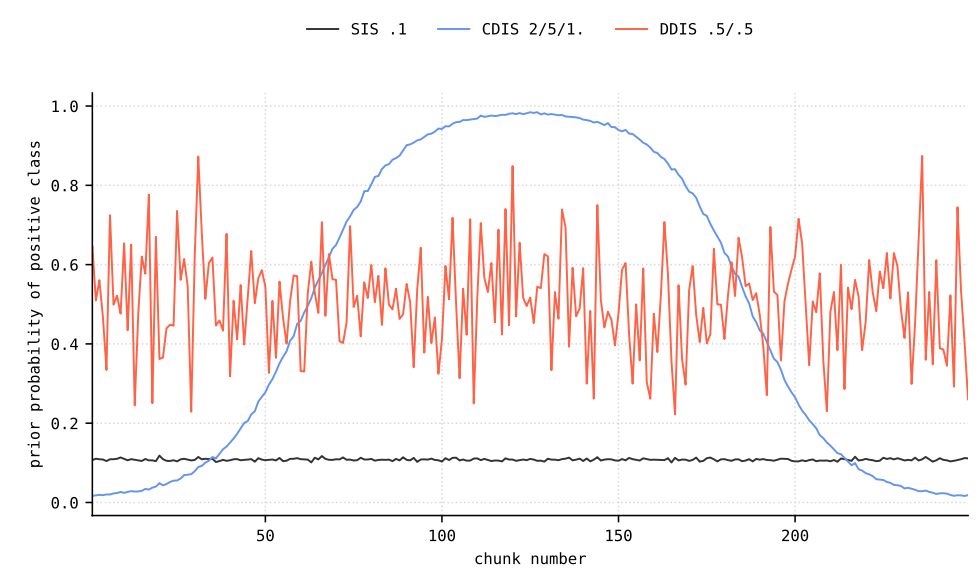
\includegraphics[width=\textwidth, clip=true]{figures/stream-taxonomy}
	\caption{Prawdopodobieństwo \emph{a priori} klasy pozytywnej dla kolejnych wsadów strumieni z każdej rozważanej kategorii strumieni niezbalansowanych.}\label{fig:stream-taxonomy}
\end{figure}

Opisywana praca -- poza taksonomią problemów -- proponuje również pulę rozwiązań standardowych oraz metodę nienadzorowanej estymacji prawdopodobieństwa \emph{a priori} zdolną do efektywnego rozpoznawania~w -- szczególnie trudnych -- strumieniach o niezbalansowaniu dyskretnie-dynamicznym (\textsc{ddis}). Algorytm \emph{Dynamic Statistical Concept Analysis} (\textsc{dsca}) wprowadza reprezentację koncepcji, jako zbioru jej standardowych miar statystycznych możliwych do wyznaczenia bez nadzoru etykiet, wraz z prostym zespołem regresorów sieci neuronowych. Modele regresji -- budowane dla każdej klasy problemu -- przy każdym kroku optymalizacji otrzymują tę samą reprezentację wsadu, jako zmienną objaśnianą przyjmując liczbę obiektów\sidenote[][-11em]{Wykorzystanie zespołu regresorów przyjmujących jako zmienną objaśnianą liczbę obiektów i integrującego końcową odpowiedź systemu przez proporcję -- w toku badań -- okazało się znacznie bardziej obiecującą strategią niż wyuczanie skali niezbalansowania. Podejście takie daje zarówno lepsze rezultaty, jak i umożliwia zastosowanie metody w~klasyfikacji wieloklasowej.} przypisanej im klasy. Zespół taki integrowany jest do wektora prawdopodobieństwa \emph{a priori} przez komplementarne skalowanie predykcji, pozwalając na późniejsze uwzględnienie w korekcie apriorycznej \textsc{pic}.

Dodatkowym elementem metody \textsc{dsca} jest dynamiczna kalibracja liczby epok uczenia, dostosowująca się do aktualnego poziomu błędu predykcji. W początkowej fazie przetwarzania wykonywanych jest więcej kroków optymalizacji -- celem szybkiego zyskania zbieżności modelu -- a z czasem wartość ta redukuje się do pojedynczych, korygujących aktualizacji (Rysunek~\ref{fig:dsca1}).

\begin{figure}[!h]
	\centering
	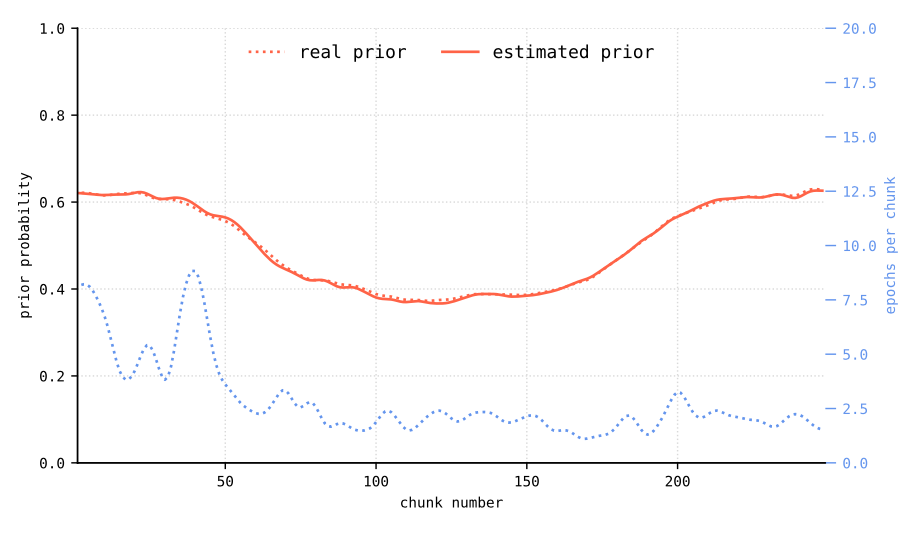
\includegraphics[width=\textwidth, clip=true]{figures/dsca1}
	\caption{Estymowane i rzeczywiste prawdopodobieństwo \emph{a priori} modelu DSCA zestawione z liczbą epok uczących regresory na wsad przetwarzania.}\label{fig:dsca1}
\end{figure}

Ewaluacja eksperymentalna metody przeprowadzona została z wykorzystaniem autorskiego generatora strumieni danych o dynamicznym niezbalansowaniu, który został zintegrowany z pakietem \emph{stream-learn}. W ramach testowanej hipotezy, badania weryfikowały możliwość zbudowania takiego modelu predykcji prawdopodobieństwa \emph{a priori}, który zdolny będzie do przewidywania w strumieniach niezbalansowanych dynamicznie w sposób dyskretny, w których standardowe podejścia będą wysoce niewydolne. Rezultaty pozwalają zaobserwować, że o ile w~wypadku strumieni niezbalansowanych statycznie nie występują istotne różnice w osiąganych rezultatach, to w niemal każdym ze scenariuszy dynamicznie-ciągłego niezbalansowania, metoda \textsc{dsca} okazuje się istotnie najlepszą w stosunku do wybranych metod referencyjnych. 

Szczególnie interesujący jest jednak przypadek wszystkich scenariuszy \textsc{ddis}, w których każda z metod referencyjnych wykazuje bardzo duży błąd -- proporcjonalny do wariancji w niezbalansowaniu. Algorytm \textsc{dsca} w takich przypadkach cechuje się bardzo wysoką efektywnością, podobną do osiąganej na pozostałych scenariuszach, okazując się jedyną dostępną obecnie w literaturze metodą odporną na niefunkcyjne zmiany w stopniu niezbalansowania.

Dalsze prace z zakresu predykcji prawdopodobieństwa \emph{a priori}, wykorzystujące zaproponowany model \textsc{dsca}, pozwoliły na uogólnienie obserwacji poczynionych wstępnie dla algorytmu \textsc{pic}, względem ogólnego modelu \emph{Multilayer Perceptron} w inkrementalnym przetwarzaniu danych.\vspace{1em}
\newpage

{
\color{red}
\noindent\begin{tabular}{p{\textwidth}}
	\toprule &
\end{tabular}\vspace{-1em}
}
\noindent Badania z zakresu przetwarzania strumieni danych często odnajdują również swoje zastosowania praktyczne. Przykładem takiego zastosowania zajmuje się praca~\citeC[-5em]{C5}, która stanowi pierwszą podjętą w literaturze przedmiotu analizę wykorzystania metod strumieniowych w zagadnieniu detekcji źródeł dezinformacji, a precyzyjnie, wykrywania treści wpisujących się w zjawisko fake news. 

Środowisko naukowe nie przyjęło jeszcze jednoznacznej i powszechnej definicji zjawiska \emph{fake news}~\citeM{Cho21}. W związku z tym, w badaniach podejmujących ten temat opieram się na określeniu go jako: \emph{treści niezgodnej z konsensusem przyjętym w określonej grupie społecznej, mającej za zadanie zmienić ten konsensus w sposób działający na niekorzyść tej grupy}.

Opisywana praca dokonuje przeglądu standardowych modeli rozpoznawania dla środowisk strumieniowych (\emph{Hoeffding Trees}, \emph{Multilayer Perceptron}, \emph{Naive Bayes}), w kontekście przetwarzania z wykorzystaniem trzech standardowych strategii budowy modeli. Analizowana jest w niej jakość (\emph{a}) modeli pojedynczych, (\emph{b}) klasycznych zespołów zbudowanych zgodnie z procedurą \textsc{sea}\sidenote[][-4em]{\emph{Streaming Ensemble Algorithm} --- podstawowy, prosty model zespołu klasyfikatorów o ustalonym limicie puli i jakościowym kryterium jej przycinania.} oraz (\emph{c}) modelu \emph{Online Bagging}, dobierającego wagi dla wzorców na podstawie rozkładu Poissona.

Ewaluacja eksperymentalna podjęta została w oparciu o zbalansowany zbiór danych \emph{Getting Real about Fake news}, zinterpretowany jako sekwencja obiektów dzięki wykorzystaniu dostępnych w nim stempli czasowych. Należy pamiętać, że typowe modele \textsc{nlp}, w procedurze wektoryzacji generują najczęściej wielowymiarowe, rozproszone macierze, które wymagają odpowiedniej redukcji wymiarowości, aby umożliwić modelowi właściwe wnioskowanie. Jest to szczególnie istotne w środowisku strumieniowym, w którym jednym z~kluczowych kryteriów jest czas przetwarzania. Każdy z modeli standardowych budowany był więc dodatkowo na zredukowanej reprezentacji problemu, wykorzystującej bazową metodę ekstrakcji w parze z (a) przycinaniem prostym po częstotliwości występowania n-gramu, (b) selekcją tokenów dokonaną przez metodę filtrową $Chi^2$ oraz (c) ekstrakcją atrybutów uzyskaną dzięki algorytmowi \emph{Principal Components Analysis}.

Przeciętnie w strumieniowym przetwarzaniu języka naturalnego prezentują się rezultaty osiągane przez pochodne algorytmu \emph{Hoeffding Tree}. Niewielkie przewagi statystyczne uzyskują one jedynie w niskowymiarowych reprezentacjach, tracąc swoją zdolność dyskryminacyjną zanim w dostępnej przestrzeni problemu pojawi się dostatecznie wiele informacji, aby uzyskać model o maksymalnej mocy. Najlepszym uzyskanym modelem przetwarzania okazał się być \emph{Multilayer Perceptron} poprzedzony analizą składowych głównych, redukującą dostępne tokeny do tysiąca niezależnych projekcji problemu, konstruujący zespół zgodnie z regułami \emph{Online Bagging}. Przy tej samej konfiguracji przetwarzania, zarówno \emph{Hoeffding Tree}, jak i podstawowy model \emph{Naive Bayes} raportowały wynik nieznacznie przekraczający poziom klasyfikatora losowego. Stanowi to dodatkowe uprawdopodobnienie hipotezy o wysokim potencjale sieci neuronowych w przetwarzaniu strumieni danych w problemach trudnych, wykraczających poza standardowe zbiory benchmarkowe o~atrybutach kategorycznych.\vspace{1em}

{
\color{red}
\noindent\begin{tabular}{p{\textwidth}}
	\toprule &
\end{tabular}\vspace{-1em}
}
\noindent Właśnie ta hipoteza stanowi główny przyczynek do analizy podjętej w~przedostatniej pracy wchodzącej w~skład cyklu~\citeC[-3.75em]{C2}. Podejmuje ona temat nienadzorowanej analizy strumieni o~atrybutach ilościowych, pozwalającej na tzw. identyfikację koncepcji.

Pierwszy istotny element pracy to propozycja \emph{sygnatury koncepcji}, czerpiąca w swojej logice z dziedziny przetwarzania sygnałów wielowymiarowych. Rysunek~\ref{fig:CS1} prezentuje przykładowe reprezentacje tego rodzaju, wyznaczone dla sześciu typowych strumieni danych zawierających dryfy koncepcji. Każdy strumień zawiera tu dwa dryfy, których punkty centralne znajdują się po trzecim i po dziewiątym wsadzie. Dla czytelności wizualizacji, strumienie zostały uproszczone do sześciu mocno skorelowanych ze sobą wymiarów, a same mapy cieplne prezentowane są jako ośmiobitowe obrazy znormalizowane odchyleniem standardowym sygnatur historycznych.

\begin{figure*}[h]
	\centering
	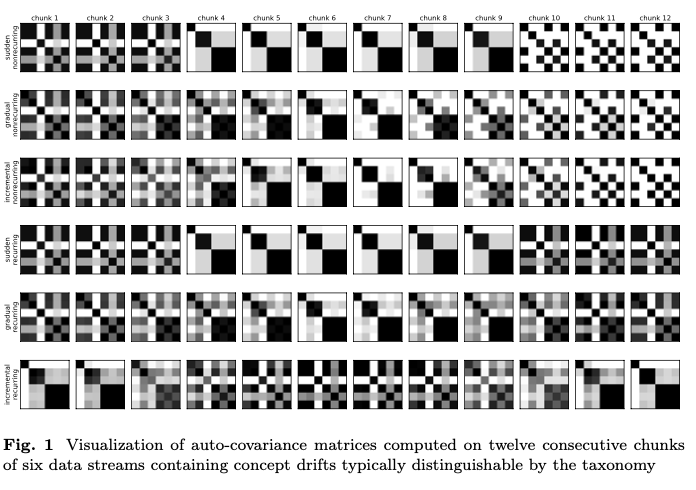
\includegraphics[width=1\textwidth, clip=true, trim=0 270 0 0]{figures/CS1}
	\caption{Wizualizacja macierzy auto-kowariancji wyznaczonych na dwunastu następujących po sobie wsadach sześciu strumieni danych zawierających dryfy koncepcji typowe dla literatury.}\label{fig:CS1}
\end{figure*}

Jak można zaobserwować, struktura zależności pomiędzy atrybutami problemu, mierzona jako ich wariancja i kros-wariancja, zmienia się proporcjonalnie do dynamiki dryfów koncepcji. W najprostszym przypadku dryfu nagłego, sygnatury koncepcji pozwalają na jednoznaczną identyfikację aktualnej interpretacji problemu. Z drugiej strony, przy dryfach inkrementalnych i gradualnych, faza przejściowa koncepcji rejestrowana jest jako płynna, stopniowa zmiana sygnatur.

Proponowana w pracy metoda \emph{Covariance-signature Concept Selector} (\textsc{cscs}) wzoruje się w swojej procedurze uczącej na takich metodach \emph{state-of-the-art}, jak \emph{Adaptive Random Forest} (\textsc{arf}), \emph{Leveraging Bagging} (\textsc{lbc}) czy \emph{Kappa Updated Ensemble} (\textsc{kue}) i również buduje zespół klasyfikatorów, ale -- w przeciwieństwie do nich -- nie integruje modeli, dokonując selekcji najbardziej odpowiedniego modelu dla aktualnie interpretowanego wsadu. Oznacza to, że inaczej niż w dotychczas stosowanych metodach, decyzja podejmowana jest zawsze przez pojedynczy model, zgodnie z paradygmatem statycznej selekcji. Co szczególnie ważne, oparcie selekcji na sygnaturach koncepcji umożliwia identyfikację koncepcji bez etykiet, a więc w obrębie procedury predykcyjnej, a tym samym, identyfikację najbardziej odpowiedniego modelu z dostępnej puli. Procedura \textsc{cscs} odrzuca standardowy paradygmat budowy zespołu, który opiera się w pozostałych metodach na zapewnieniu modeli o możliwie najwyższej jakości i różnorodności, zastępując go paradygmatem najwyższego podobieństwa pomiędzy problemem i jego predyktorem. Taka zmiana pozwala zarówno na identyfikację nowych koncepcji, jak i na selekcję modelu odpowiedniego dla aktualnego, nieoznaczonego wsadu.

Metoda \textsc{cscs} została poddana szerokiej ewaluacji eksperymentalnej, uwzględniającej zarówno osiem metod \emph{state-of-the-art} (z trzech generacji zespołowych algorytmów przetwarzania strumieni), jak i trzy kategorie scenariuszy testowych: 

\begin{itemize}
	\item Dwa z nich uwzględniają ewaluację na danych syntetycznych -- pochodzących zarówno z generatorów \textsc{moa}, jak i generatora \emph{stream-learn}
	\item Trzeci opiera się na strumieniach pół-syntetycznych, wstrzykujących dryfy do koncepcji rzeczywistych, pozwalając na ustrumieniowienie problemów stacjonarnych~\citeM{Kom22b}\marginnote{Strategia ta opisana została w osobnym artykule, przyjętym do publikacji na konferencji ESANN'22, na którą przygotowaliśmy krótki film prezentujący zasadę działania generatora strumieni.\\\noindent\url{https://youtu.be/00KEJXAQrt8}}.	
\end{itemize}

Dodatkowo, jako modele bazowe dla eksperymentów przyjęto zarówno \emph{Hoeffding Tree} (w implementacji \textsc{cvfdt}), jak i \emph{Multilayer Perceptron}. Podejście takie pozwoliło na odpowiednią analizę zachowania wszystkich rozważanych metod w problemach o różnej charakterystyce atrybutów (ilościowe, jakościowe i hybrydowe) przy różnych bazowych modelach klasyfikacji.

%Uzyskane rezultaty (Tabela~\ref{tab:CSCS}) pozwalają na identyfikację jednoznacznych trendów w przetwarzaniu. Stanowiący obecnie \emph{state-of-the-art} dziedziny algorytm \emph{Leverage Bagging Clasifier} -- zgodnie z przewidywaniami i raportami dostępnymi w literaturze -- okazuje się budować modele istotnie przewyższające konkurencję w wypadku strumieni o atrybutach jakościowych. Analogicznie jak w podobnej do niego metodzie \emph{Adaptive Random Forest}, nie stosuje się go jednak w kombinacji z innymi klasyfikatorami bazowymi niż drzewa Hoeffdinga, co utrudnia mu osiąganie wysokich rezultatów w wypadku problemów o cechach jakościowych. Wykonując tę analizę wyłącznie w oparciu o drzewa Hoeffdinga należałoby jednoznacznie przyjąć jego przewagę nad pozostałymi rozważanymi metodami rozpoznawania, ale byłoby to działanie pochopne -- pomijające ograniczenia metod drzewiastych w przetwarzaniu danych ilościowych.

Globalna analiza, uwzględniająca również perceptron wielowarstowy, pokazuje, że w wypadku wszystkich strumieni ilościowych, połączenie \emph{Multilayer Perceptron} i \textsc{cscs} wykazuje istotną przewagę statystyczną zarówno nad wszystkimi pozostałymi metodami rozpoznawania opartymi o sieci neuronowe, jak i względem modeli opartych o \emph{Hoeffding Tree}.

Podobnie prezentują się wyniki osiągnięte dla strumieni pół-syntetycznych. W wypadku niskiej wymiarowości, w których sygnatura koncepcji jest niewielka i nie uzyskuje jeszcze pełnego potencjału różnicującego, pewną przewagę nad \textsc{cscs} wykazują jeszcze modele \textsc{arf} i \textsc{lbc}. Po przekroczeniu czterech wymiarów problemu, sygnatury \textsc{cscs} pozwalają już na właściwą identyfikację i budują modele sieci neuronowych statystycznie istotnie lepsze od każdego z pozostałych testowanych rozwiązań. 

Dodatkową właściwością \textsc{cscs} jest minimalizacja narzutu obliczeniowego niezbędnego do konstrukcji modelu o dużej zdolności dyskryminacyjnej. Jak można zaobserwować na Rysunku~\ref{fig:wegiel}, proponowana przeze mnie metoda wykazuje minimalnie większą złożoność jedynie względem najstarszego i najprostszego zespołu strumieniowego -- \emph{Streaming Ensemble Algorithm}. Ponadto, model ten, kiedy oparty jest o~\emph{Multilayer Perceptron}, wykazuje o~rząd niższą złożoność obliczeniową niż bazowy model \emph{Hoeffding Tree} w problemach wielowymiarowych, prezentując się jako niezwykle skuteczne narzędzie w~przetwarzaniu wielowymiarowych strumieni danych o~charakterystyce ilościowej.

\begin{figure}[!htb]
	\centering
	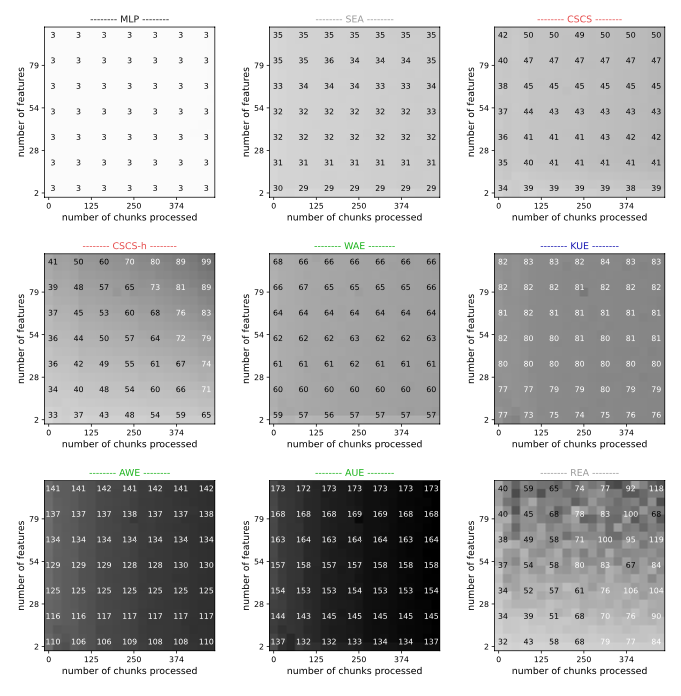
\includegraphics[width=1\textwidth, clip=true]{figures/wegiel}
	\caption{Czas (w milisekundach) wymagany do przetworzenia pojedynczego wsadu przez różne metody zespołowe wykorzystujące \temph{Multilayer Perceptron} w zależności od liczby przetworzonych wsadów i wymiarowości problemu.}\label{fig:wegiel}
\end{figure}

\vspace{1em}
\newpage
{
\color{red}
\noindent\begin{tabular}{p{\textwidth}}
	\toprule &
\end{tabular}\vspace{-1em}
}
\noindent Zagadnienie identyfikacji zmian koncepcji, przyjmując już bardziej typowe podejście wykorzystujące detektory dryfów i przebudowę modeli bez identyfikacji rozkładu, rozważałem również w pracy~\citeC[-5em]{C1}.

W pracy tej proponowany jest efektywny zespół detektorów dryfu \emph{Statistical Drift Detection Ensemble} (\textsc{sdde}), oparty na statystycznych miarach \emph{drift magnitude} oraz \emph{conditioned marginal covariate drift}, stanowiący przykład detektora agnostycznego, tj. niezależnego od odpowiedzi klasyfikatora. Należy zaznaczyć, że nie oznacza to budowy modelu nienadzorowanego, ponieważ wykorzystuje on etykiety obiektów do budowy reprezentacji wiedzy o rozkładzie klas, ale nie uzależnia swoich decyzji od zmian jakości klasyfikacji w funkcji czasu, jak robią to klasyczne detektory dryfu.

Miara \emph{drift magnitude} definiowana jest przez dystans pomiędzy koncepcjami w punktach w czasie $t$ i $u$, rozumiana jako dystans pomiędzy rozkładami atrybutów $P(X)$ w tychże

\begin{equation}
	DM_{t,u} = D(P_t(X), P_u(X)),
\end{equation}

\noindent gdzie dystans pomiędzy rozkładami estymowany jest przez metrykę Hellingera.

Druga wykorzystana miara, \emph{conditioned marginal covariance drift} definiowana jest jako ważona suma odległości pomiędzy warunkowymi rozkładami prawdopodobieństwa dla możliwych kategorii $P(X|Y)$ pomiędzy punktami w czasie $t$ i $u$. Wagi stanowią średnie prawdopodobieństwa wystąpienia obiektów danej klasy $P(Y)$ w obu punktach w~czasie

\begin{equation}
	\sigma_{t,u}^{X|Y} = \sum_{y\in Y} \Big[ \frac{P_t(y)+P_u(y)}{2} \frac{1}{2} \sum_{y\in Y} |P_t(\bar{x}|y)-P_u(\bar{x}|y)| \Big].
\end{equation}

W metodzie \textsc{sdde} miary nie są wyliczane na pełnej wymiarowości strumienia, a jedynie na jego podprzestrzeniach, czyniąc z niej rozwiązanie dedykowane strumieniom wielowymiarowym. Rozbicie problemu na podprzestrzenie nie tylko pozwala uniknąć problemów wynikających z klątwy wielowymiarowości, ale także zapewnia zespół detektorów w~miejsce pojedynczego narzędzia pomiarowego. W~jednej z wcześniejszych prac zespołu zauważyliśmy, że klasyczne metody integracji puli -- typowe dla zadania klasyfikacji -- nie przynoszą tak dobrych rezultatów w detekcji dryfu~\citeM{Woz16}, w~związku z czym dla \textsc{sdde} zaproponowana została integracja dwupoziomowa. W~ramach detektorów bazowych, zbudowanych w~obrębie tej samej podprzestrzeni), decyzja podejmowana jest na podstawie porównania aktualnych wartości metryk ze średnią harmoniczną wartości historycznych, opierając się na regule trzy-sigma. Integracja podprzestrzeni odbywa się już przez hiperparametr progu wzbudzenia, dobrany eksperymentalnie dla analizowanych strumieni. Przykład przetwarzania algorytmu \textsc{sdde} zaprezentowany został na Rysunku~\ref{fig:sdde}.

\begin{figure}[!htb]
	\centering
	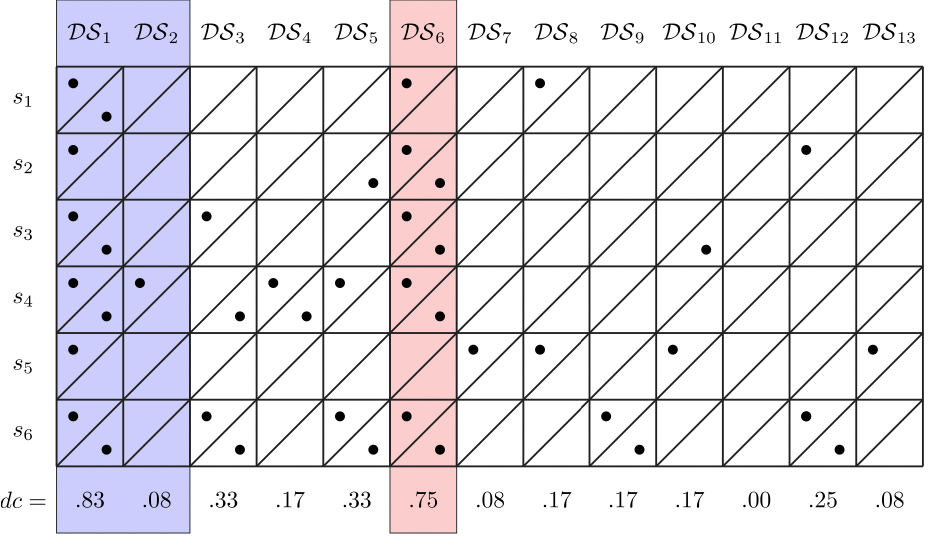
\includegraphics[width=\textwidth, clip=true]{figures/sdde}
	
\begin{enumerate}
	\item Początkowa faza przetwarzania, zaznaczona kolorem niebieskim, stanowi okres unieruchomienia wzbudzeń, w których niezależnie od odpowiedzi detektorów, zespół wskazuje na stabilność koncepcji. 
	\item Jednostkowe wzbudzenia detektorów bazowych -- oznaczone czarnymi kropkami -- nie prowadzą do przebudowania informacji o rozkładach, informując jedynie o aktualnym stanie odległości pomiędzy rozkładem pierwotnym i aktualnym.
	\item Osiągnięcie progu wzbudzenia zespołu -- zaznaczone na czerwono -- prowadzi do wyzwolenia aktualizacji modelu, zapisania informacji o~aktualnym rozkładzie w każdej podprzestrzeni i wykorzystywaniu jej jako punktu odniesienia w nadchodzących wsadach aż do momentu kolejnej detekcji dryfu.
\end{enumerate}


	\caption{Przykład przetwarzania algorytmu \emph{Statistical Drift Detection Ensemble}. Kolejne kolumny prezentują kolejne analizowane wsady, kolejne wiersze to następujące po sobie pary detektorów. Punkt oznacza wzbudzenie pojedynczego detektora, obszar niebieski -- interwał ochronny zespołu detektorów, a obszar czerwony -- wsad, w którym zespół identyfikuje dryf koncepcji. Opis procedury znajduje się w punktach poniżej ilustracji.}\label{fig:sdde}
\end{figure}

Za estymator rozkładów prawdopodobieństwa w każdym z niezbędnych elementów przyjęto jądrową estymację gęstości (\emph{Kernel Density Estimation}).

Istotnym uzupełnieniem pracy była propozycja korekty w standardowym podejściu do analizy efektywności detektorów dryfu. Jak zostało to już zauważone w literaturze, odradza się ewaluację detektorów wyłącznie w oparciu o jakość klasyfikacji, ponieważ podejście takie nie tylko utrudnia wyciąganie właściwych wniosków z badań, ale nawet promuje metody losowo przebudowujące modele co zadany interwał. Przedstawiona propozycja stanowi zbiór trzech metryk uzupełniających:

\begin{itemize}
	\item[$D_1$] -- miara najbliższego dryfu -- średnia odległość każdej detekcji od najbliższego dryfu.
	\item[$D_2$] -- miara najbliższej detekcji -- średnia odległość każdego rzeczywistego dryfu do najbliższej detekcji.
	\item[$R$] -- współczynnik dryfu do detekcji -- skalowana do zera w wartości oczekiwanej i wyznaczana z wartości bezwzględnej proporcja pomiędzy liczbą dryfów i detekcji.
\end{itemize}

Zrealizowana ewaluacja eksperymentalna pozwoliła na zweryfikowanie algorytmu \textsc{sdde} jako efektywnego narzędzia detekcji dryfu, w~szczególności w przypadkach trudnych. W~ramach oceny zwalidowano jego jakość w zestawieniu z metodami \emph{state-of-the-art} takimi jak \textsc{hddm} (w odmianach \textsc{hddm}$_A$ i \textsc{hddm}$_W$) czy \textsc{adwin}, oraz z klasycznymi detektorami \textsc{ddm} i \textsc{eddm}. Jak można zauważyć na reprezentatywnym przypadku (Rysunek~\ref{fig:sdde2}), detektor ten nie tylko pozwala na jednoznaczną identyfikację dryfu w czytelnym scenariuszu dryfu nagłego, gdzie jedynie algorytmy \textsc{hddm}$_w$ i \textsc{adwin} były zdolne do nawiązania z nim konkurencji, ale i w dryfach gradualnych, pozwalając na rozpoznanie zmian już w początkowej fazie dryfu, informując model na bieżąco o ich dynamice -- podobnie jak metoda \textsc{cscs} -- będąc czułym nie tylko na stabilne koncepcje główne, ale też na każdą z koncepcji pośrednich.

\begin{figure}[!htb]
	\centering
	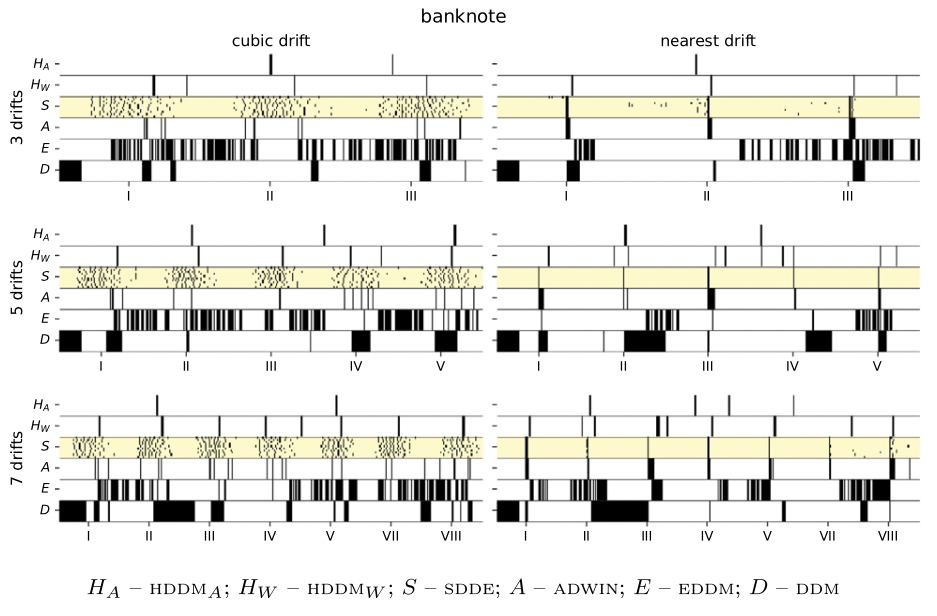
\includegraphics[width=\textwidth, clip=true, trim= 0 400 0 0]{figures/sdde2}
	\caption{Przykładowy wynik ewaluacji metody \emph{Statistical Drift Detection Ensemble} (na żółto) w scenariuszu półsyntetycznym.}\label{fig:sdde2}
\end{figure}

\subsection{Podsumowanie osiągnięcia naukowego i kierunki dalszych badań}

Prace opisane w ramach zaprezentowanego cyklu publikacji stanowią podsumowanie kolekcji metod pozwalających modelom klasyfikacji rozwiązywać szerokie spektrum problemów, w których często niemożliwe jest efektywne zastosowanie typowych rozwiązań znanych z literatury, a~nawet algorytmów \emph{state-of-the-art}. 

Koncentracja trudności, przykładowo, w wielowymiarowych strumieniach danych wykazujących zarówno dryf koncepcji, jak i dynamiczne niezbalansowanie o charakterystyce uniemożliwiającej jego funkcyjną analizę\sidenote{Strumienie niezbalansowane kategorii \textsc{ddis}}, wymaga metod specyficznych, radzących sobie z wieloma wyzwaniami równocześnie. Zaproponowany przeze mnie zbiór algorytmów stara się wychodzić tym trudnościom naprzeciw, wykazując w większości przypadków statystycznie istotnie lepsze wyniki nad rozwiązaniami znanymi z literatury, zalecanymi często do typowych problemów, dostosowanymi do ogólnych przypadków klasyfikacji danych trudnych, ale przez to też niezdolnymi do efektywnego przetwarzania w przypadkach skrajnych.

Podczas projektowania eksperymentów takiego właśnie scenariusza~\citeC{C7}, większość implementacji wykorzystywanych w badaniach trudnych strumieni danych opierała się na frameworku \textsc{moa}, stanowiącym ówczesny standard badawczy dla rozwiązań uczenia online, przeprowadzanych zgodnie z protokołem \emph{Prequential Analysis}, opierając modele na odmianach \emph{Hoeffding Tree}. Pakiet ten nie udostępniał jednak interfejsu programistycznego pozwalającego na badania z zakresu uczenia aktywnego, a więc konieczne było opracowanie dodatkowego oprogramowania pozwalającego na stosowną analizę.

Ze względu na rosnącą ówcześnie popularność pakietu \emph{scikit-learn} i~języka Python w środowisku badań nad sztuczną inteligencją, rozpocząłem prace nad nową biblioteką -- nastawioną na przetwarzanie wsadowe i ewaluację uwzględniającą ilościową naturę danych strumieniowych. Jej~pierwsza wersja rozwojowa użyta została jako podstawa do ówcześnie realizowanych badań, a stabilna wersja została opublikowana wraz z~artykułem towarzyszącym w~czasopiśmie Neurocomputing, w~styczniu 2022 roku~\citeM{Ksi22a}.

Takie podejście do badań sprawia, że zaproponowane rozwiązania nie stanowią jedynie rozważań teoretycznych, ograniczonych do odseparowanych środowisk eksperymentowania, ale w dominującej większości są dostępne dla społeczności akademickiej w formie zoptymalizowanych i~udokumentowanych implementacji wchodzących w~skład dostępnych w publicznych repozytoriach pakietów oprogramowania \emph{stream-learn}, \emph{weles} i \emph{problexity}.

\begin{itemize}
	\item \emph{Stream-learn — open-source Python library for difficult data stream batch analysis}\\%\marginnote[0em]{\noindent
\includegraphics[width=1.5cm]{WoS.png}}
	
	\url{https://github.com/w4k2/stream-learn}\\
	\url{https://stream-learn.readthedocs.io}\\
	\newpage
	
	\item \emph{Weles — Collection of pattern recognition methods and experimental tools made by ML Group of Wrocław University of Science and Technology.} \\%\marginnote[0em]{\noindent
\includegraphics[width=1.5cm]{WoS.png}}
	
	\url{https://github.com/w4k2/weles}\\
	\url{https://weles.readthedocs.io}\\

	\item \emph{Problexity — an open-source python library containing the implementation of measures describing the complexity of the classification problem.} \\%\marginnote[0em]{\noindent
\includegraphics[width=1.5cm]{WoS.png}}
	
	\url{https://github.com/w4k2/problexity}\\
	\url{https://problexity.readthedocs.io}\\	\vspace{1em}
\end{itemize}
 
 Pozwala to zarówno na replikację prezentowanych rezultatów badań, jak i dalszy ich rozwój, umożliwiający inkrementalne ulepszanie rozwiązań dedykowanych klasyfikacji danych trudnych. 
 Wśród metod, które zaproponowałem w pracach wchodzących w skład cyklu należy wymienić:

\begin{itemize}
	\item \textbf{Metodę\marginnote{\emph{dane wielowymiarowe}} zespołowej klasyfikacji obrazów nadwidmowych w oparciu o Extreme Learning Machines} -- algorytm pozwalający na wykorzystanie, szczególnie pożądanego w praktycznych aplikacjach (w~zagadnieniu rolnictwa precyzyjnego czy kontroli jakości), podejścia ręcznej inżynierii atrybutów projekcyjnych przy zastosowaniu szybko uczących się modeli neuronowych.
	\item[]\vspace{-.5em} \emph{\color{red}\footnotesize\fullcite{C10}}
	 
	\item \textbf{Genetyczną\marginnote{\emph{dane wielowymiarowe}\\\noindent\emph{dane niezbalansowane}} metodę doboru zespołu klasyfikatorów w środowisku niezbalansowanych danych wielowymiarowych} -- metodę pozwalającą na optymalizację efektywności modeli w problemach niezbalansowanych o liczności klasy mniejszościowej uniemożliwiającej syntetyczne balansowanie problemu.\\
	\item[]\vspace{-.5em} \emph{\color{red}\footnotesize\fullcite{C9}}
	
	\item \textbf{\emph{Exposer\marginnote{\emph{dane wielowymiarowe}\\\noindent\emph{dane niezbalansowane}} Classifier Ensemble}} -- zespołową metodę klasyfikatora bazowego, odporną na klątwę wielowymiarowości i niezależną od stopnia niezbalansowania problemu przy jednoczesnym zachowaniu braku zależności statystycznej względem typowych modeli rozpoznawania. 
	\item[]\vspace{-.5em} \emph{\color{red}\footnotesize\fullcite{C11}}
	
	\item \textbf{\emph{Subspace-driven\marginnote{\emph{dane wielowymiarowe}\\\noindent\emph{dane niezbalansowane}} SMOTE}} -- architekturę zespołu klasyfikatorów przesuwającą fazę przetwarzania wstępnego do -- zdatnego do krzyżowej oceny i dodatkowej kalibracji -- zbioru podprzestrzeni problemu, redukujących negatywne skutki klątwy wielowymiarowości. 
	\item[]\vspace{-.5em} \emph{\color{red}\footnotesize\fullcite{C6}}
	
	\item \textbf{\emph{Undersampled\marginnote{\emph{dane niezbalansowane}} Majority Class Ensemble}} -- architekturę zespołu klasyfikatorów dedykowaną danym silnie niezbalansowanym, pozwalającą na pełne wykorzystanie dostępnych obiektów problemu, bez konieczności wprowadzania do przetwarzania obiektów syntetycznych.
	\item[]\vspace{-.5em} \emph{\color{red}\footnotesize\fullcite{C8}}
	
	\item \textbf{Metodę\marginnote{\emph{strumienie danych}} aktywnego przetwarzania strumieni danych opartą o~\emph{Relative Support Function Difference}} -- pozwalającą na racjonalizację kosztu pozyskiwania stronniczości eksperckiej w~problemach o~zmiennym prawdopodobieństwie \emph{a posteriori}.
	\item[]\vspace{-.5em} \emph{\footnotesize\color{red}\fullcite{C7}}
	
	\item \textbf{\emph{Prior\marginnote{\emph{dane niezbalansowane}\\\noindent\emph{strumienie danych}} Imbalance Compensation}} -- agnostyczną procedurę pozwalającą na zwiększenie mocy dyskryminacyjnej modeli klasyfikacji w strumieniach niezbalansowanych bez konieczności stosowania przetwarzania wstępnego, metod wbudowanych ani hybrydowych.  
	\item[]\vspace{-.5em} \emph{\footnotesize\color{red}\fullcite{C4}}
	
	\item \textbf{\emph{Dynamic\marginnote{\emph{dane niezbalansowane}\\\noindent\emph{strumienie danych}} Statistical Concept Analysis}} -- rozwinięcie metody \textsc{pic} o~efektywny estymator prawdopodobieństwa \emph{a priori}, zdolny do osiągania wysokiej efektywności nawet w skrajnych przypadkach strumieni o niezbalansowaniu dyskretnie-dynamicznym.
	\item[]\vspace{-.5em} \emph{\footnotesize\color{red}\fullcite{C3}}
	
	\item \textbf{\emph{Covariance-signature\marginnote{\emph{dane wielowymiarowe}\\\noindent\emph{dane niezbalansowane}\\\noindent\emph{strumienie danych}} Concept Selector}} -- zespołową metodę klasyfikacji trudnych strumieni danych o cechach ilościowych, dedykowaną przetwarzaniu z wykorzystaniem modeli sieci neuronowych.
	\item[]\vspace{-.5em} \emph{\footnotesize\color{red}\fullcite{C2}}
	
	\item \textbf{\emph{Statistical\marginnote{\emph{strumienie danych}} Drift Detection Ensemble}} -- zespołowy detektor dryfu dedykowany rozpoznawaniu zmian w rozkładach \emph{a posteriori} dla strumieni wielowymiarowych, stanowiący metodę agnostyczną -- niezależną od wykorzystywanego modelu klasyfikacji.
	\item[]\vspace{-.5em} \emph{\footnotesize\color{red}\fullcite{C1}}
	 
\end{itemize}


\noindent Oprócz tematyki zawartej w prezentowanym cyklu moje zainteresowania naukowe dotyczą również innych tematów sztucznej inteligencji. Zagadnienie detekcji źródeł dezinformacji i klasyfikacji \emph{fake news}, który poruszyłem tu w kontekście przetwarzania strumieniowego, rozwijam w kolejnych pracach analitycznych, w których znajdują się zarówno propozycje nowych algorytmów, jak i najaktualniejszy obecnie artykuł przeglądowy~\citeM[-4em]{Cho21} stanowiący zbiór punktów wyjścia dla prac prowadzonych w ramach kierowanego przeze mnie projektu \textsc{swarog}\footnote{Na tropie fake newsów, czyli projekt \textsc{swarog}\\\noindent\url{https://wit.pwr.edu.pl/aktualnosci/na-tropie-fake-newsow-\\-czyli-projekt-swarog-5.html}}.


Zagadnienie przetwarzania strumieni danych analizuję również w~kontekście zespołowych detektorów dryfu, strumieni niezbalansowanych skrajnie, modyfikacji standardowych metryk ważenia zespołów klasyfikatorów, dalszych prac nad uczeniem aktywnym czy oceny potencjału balansowania strumieni. 

Dane niezbalansowane analizuję też nadal w ich stacjonarnej odmianie, zarówno dla danych sygnałowych jak i tabelarycznych, uwzględniając tu zarówno wątek integracji geometrycznej~\citeM{Ksi21k} jak i potencjału algorytmów genetycznych w dywersyfikacji zespołów. Podobnie, rozwijam też wątek przetwarzania danych wielowymiarowych, zarówno w~ujęciu tabelarycznym, jak i sygnałowym.

Ponadto, w swoich badaniach przykładam szczególną wagę do poprawności protokolarnej, o czym świadczyć może moje współautorstwo w pracy przeglądowej przedstawiającej dobre praktyki projektowania rzetelnych eksperymentów~\citeM[-2em]{Sta21}. Opisane przedsięwzięcie stanowi zarówno odpowiedź na aktualne i podlegające intensywnym badaniom problemy, jak i zbiór stabilnych rozwiązań, możliwych do zastosowania i~stosowanych w rzeczywistych problemach.

\newthought{Wykorzystana literatura pomocnicza}

{\footnotesize
\begin{fullwidth}
\begin{itemize}
	\item[[Z1]] \fullcite{Z1}
	\item[[Z2]] \fullcite{Z2}
	\item[[Z3]] \fullcite{Z3}
	\item[[Z4]] \fullcite{Z4}
	\item[[Z5]] \fullcite{Z5}
	\item[[Z6]] \fullcite{Z6}
	\item[[Z7]] \fullcite{Z7}
	\item[[Z8]] \fullcite{Z8}
	\item[[Z9]] \fullcite{Z9}
	\item[[Z10]] \fullcite{Z10}
	\item[[Z11]] \fullcite{Z11}
	\item[[Z12]] \fullcite{Z12}
	\item[[Z13]] \fullcite{Z13}
	\item[[Z14]] \fullcite{Z14}
	\item[[Z15]] \fullcite{Z15}
	\item[[Z16]] \fullcite{Z16}
	\item[[Z17]] \fullcite{Z17}
	\item[[Z18]] \fullcite{Z18}
	\item[[Z19]] \fullcite{Z19}
	\item[[Z20]] \fullcite{Z20}
	\item[[Z21]] \fullcite{Z21}
	\item[[Z22]] \fullcite{Z22}
	\item[[Z23]] \fullcite{Z23}
	\item[[Z24]] \fullcite{Z24}
	\item[[Z25]] \fullcite{Z25}
	\item[[Z25]] \fullcite{Z26}
\end{itemize}
\end{fullwidth}
}